\documentclass[12pt,oneside,a4paper]{article}
\usepackage[utf8]{inputenc}
\renewcommand{\familydefault}{\sfdefault}
\usepackage[a4paper,left=3cm,right=3cm,top=3cm,bottom=3cm]{geometry}
\usepackage{todonotes}
\usepackage[english,german]{babel} 
\usepackage{pdfpages}
\usepackage{multirow}
\usepackage{tabularx}
\usepackage{makecell}
\usepackage{graphicx}
\usepackage{titleref}
\usepackage{csquotes}

\setlength {\marginparwidth }{2cm}
\setlength{\parindent}{0pt}

\usepackage[skip=0.5\baselineskip]{caption}
\usepackage{newtxtext,newtxmath}
\usepackage{float}
\usepackage[style=apa,
backend=biber,
maxbibnames=99,
sorting=none]{biblatex} 
\usepackage{hyperref}
\hypersetup{
    colorlinks,
    citecolor=black,
    filecolor=black,
    linkcolor=black,
    urlcolor=black
}
\usepackage{titlesec}
\titleformat*{\section}{\Large\bfseries}
\titleformat*{\subsection}{\Large\bfseries}
\titleformat*{\subsubsection}{\large\bfseries}
\titleformat*{\paragraph}{\large\bfseries}
\titleformat*{\subparagraph}{\large\bfseries}
\usepackage{fancyhdr}
\fancyhf{}
\renewcommand{\headrulewidth}{0pt}
\rfoot{\thepage}
\lfoot{Kooperation in VR auf Basis von ViRGOS}

\addbibresource{references.bib} 
\DeclareFieldFormat[article,inbook,InProceedings]{title}{#1} 

\pagestyle{fancy}
\begin{document}
\large
\begin{titlepage}
	\centering
	
\includegraphics[width=0.5\textwidth]{LogoReutlingen.png}\par\vspace{1cm}
	\vspace{0.5cm}
	{\Large Bachelor-Thesis\par}
	\vspace{1.5cm}
	{\huge\bfseries Kooperation in Virtual Reality auf Basis von ViRGOS\par}
	\vspace{2cm}
	{\Large\bfseries Eine Erweiterung der ViRGOS-Anwendung um Mehrspieler-Funktionalitäten mit dem Ziel der asymmetrischen Kooperation \par}
	\vspace{2cm}
	{Marcel Neumann, 764541 \\ marcel.neumann@student.reutlingen-university.de\\
	\vspace{1cm}
	Erstprüfer: Prof. Dr. Uwe Kloos\\
	Zweitprüferin: Prof. Dr. Gabriela Tullius\\
	\vspace{0.2cm}
	\par}
	\vfill
{\large 
Hochschule Reutlingen\\
Fakultät Informatik\\
Medien- und Kommunikationsinformatik\\
\vspace{1cm}
30. Juni 2020}
\end{titlepage}


\section*{\centering{Zusammenfassung}}
ViRGOS ist eine bestehende Virtual Reality Anwendung der Hochschule Reutlingen. Diese Arbeit beschäftigt sich mit der Erweiterung dieser Anwendung, mit dem Ziel mehreren Spielern die Möglichkeit der asymmetrischen Kooperation zu bieten. In dieser Anwendung nehmen Benutzer zwei unterschiedliche Rollen ein. Ein Benutzer löst eine Aufgabe, während er von einem anderen angeleitet wird, wodurch es zu einer Asymmetrie in der Kooperation kommt. Es werden Anforderungen an die Erweiterung definiert und Funktionen und Werkzeuge konzeptioniert, um diese Kooperation zu ermöglichen. Der größte Teil der Konzeption kann umgesetzt werden, sodass die asymmetrische Kooperation in der Anwendung möglich ist. Um die qualitative Umsetzung zu testen, wird eine kleine Expertenbefragung durchgeführt und in dieser Arbeit ausgewertet.\\ \todo{Eventuell Umfrage Ergebnisse rein?}

Im Anhang befindet sich ein einfacher Fragebogen der für eine größere Probandenbefragung konzipiert wurde, die aufgrund der Covid-19-Pandemie leider nicht durchgeführt werden kann.

\begin{otherlanguage}{english}
\section*{\centering{Abstract}}
ViRGOS is an existing virtual reality application of Reutlingen University. This work deals with the extension of this application, with the goal to offer several players the possibility of asymmetrical cooperation. In this application, users take on two different roles. One user solves a task while being guided by another, which leads to an asymmetry in the cooperation. The requirements for this extension are defined and functions and tools are designed to enable this cooperation. Most of the conception can be implemented, so that asymmetric cooperation in the application is possible. In order to test the qualitative implementation, a small expert survey is conducted and evaluated in this thesis.\\

The appendix contains a simple questionnaire which was designed for a larger survey, which unfortunately cannot be carried out due to the Covid-19 pandemic.
\end{otherlanguage}

\newpage

\tableofcontents

\newpage
\listoffigures
\section{Einleitung}
Dieses Kapitel beleuchtet zuerst die allgemeine Problemstellung mit der sich in dieser Arbeit auseinander gesetzt wird. Anschließend wird die Anwendung ViRGOS erklärt, die als Grundlage für diese Arbeit dient. Abschließend wird die Struktur der kompletten Arbeit in Form der einzelnen Kapitel erklärt.

\subsection{Problemstellung und Motivation} \label{Problemstellung}
https://lehrerfortbildung-bw.de/u_gewi/religion-rk/gym/bp2004/fb1/1_theorie/komp/2_konstrukt/#46
Aus eigener Erfahrung ist bekannt, dass sich Dinge leichter erlernen lassen wenn man sie anwendet, statt über sie zu lesen oder sie erklärt zu bekommen. Besonders praktische Prozeduren müssen durchgeführt und geübt werden, um vollkommen erlernt zu werden. Virtual Reality bietet hierbei vielversprechende Möglichkeiten um sowohl theoretisches Wissen durch Visualisierung, als auch praktisches Wissen durch Anwendung zu vermitteln. Mehrere Studien bestätigen das Potential, das Virtual Reality als Bildungswerkzeug birgt. ~\parencite{8864531} ~\parencite{8797755} Des Weiteren ermöglicht Virtual Reality die Kollaboration über größere Distanzen. In einer zunehmend globalisierten und digitalisierten Gesellschaft ist Zusammenarbeit mit Personen in anderen Standorten keine Seltenheit. Dies kann jedoch zu Problemen führen, wenn Unterstützung eines Experten mit spezifischem Fachwissen benötigt wird. Insbesondere bei praktischen Prozessen, die Demonstrationen bedürfen, stellt die Entfernung eine große Hürde dar. Bei diesen Unterrichtungs- und Fernwartungsszenarien über große Distanzen bietet Virtual Reality eine vielversprechende Abhilfe. ~\parencite{10.1145/2807442.2807497} Bei diesen asymmetrischen Kollaborationen verfügt einer der Benutzer über größeres Wissen als ein oder mehrere andere. Dieser Benutzer fungiert als Lehrer und versucht sein Wissen mittels der Anwendung an die anderen Benutzer weiterzugeben. \\


\subsection{Ziel der Arbeit}

Das Ziel der Arbeit ist die bestehende Anwendung der Hochschule zu erweitern und mehreren Benutzern zeitgleich Zugriff zu gewähren. Die Benutzer sollen hierbei miteinander Interagieren und asymmetrisch Kooperieren können, um eine gemeinsame Aufgabe zu lösen. Die Asymmetrie soll durch die zwei Rollen Kommandant und Astronaut hervorgerufen werden, die die Benutzer einnehmen sollen. Der Kommandant soll den Astronauten als Experte bei der Aufgabe unterstützen. Hierfür sollen dem Kommandanten mehrere Werkzeuge zur Kommunikation zur Verfügung stehen. \\

Hieraus ergibt sich folgende Forschungsfrage:

\begin{itemize}
\item[FF1] \label{FF1} Welche Funktionalitäten muss eine VR Anwendung bieten, um die asymmetrische Kollaboration zu ermöglichen?
\end{itemize}

Es soll also festgestellt werden, welche Funktionalitäten unabdingbar für die Kooperation sind. Außerdem soll untersucht werden, welche Werkzeuge den Benutzern am meisten helfen ihre Aufgabe gemeinsam zu lösen.


\subsection{Struktur der Arbeit}
Das erste Kapitel dient als Einleitung und schildert die Problemstellung, mit der sich in dieser Arbeit befasst wird. Außerdem wird ViRGOS als Grundlage für die Arbeit erläutert und der Ist-Zustand der Anwendung vor Beginn der Entwicklung erklärt. \newline

Der Stand der Wissenschaft bezüglich der Thematik wird in Kapitel zwei beschrieben. Hier wird auf verwandte Literatur eingegangen, die sich mit dem Einsatz von Virtual Reality zur Vermittlung von Wissen und der Kooperation mehrerer Nutzer beschäftigt. \newline

Kapitel drei beschäftigt sich mit der Konzeption der Anwendung. Zu Beginn werden die Anforderungen an das Projekt analysiert. Anschließend wird eine Auswahl aus mehreren Technologien getroffen, die in diesem Projekt zum Einsatz kommen könnten. Im Anschluss wird das Konzept eines Prototypen und der eigentlichen Anwendung erklärt. Es wird auf die Mehrspielerfähigkeit von ViRGOS eingegangen und geplante Werkzeuge beschrieben. Zum Abschluss wird auf Tests der Anwendung und Befragungen von Probanden eingegangen. \newline

Wie die geplanten Funktionalitäten umgesetzt wurden ist Thema des vierten Kapitels. Als Erstes wird erklärt wie der Prototyp entwickelt wurde und zu was dieser fähig ist. Im nächsten Unterkapitel werden die Implementierungen der Funktionen von ViRGOS geschildert. Abschließend wird auf Einschränkungen eingegangen, die durch die Gesundheitslage zum Zeitpunkt der Erstellung dieser Arbeit bestand. \newline

Kapitel 5: Probandenbefragung \todo{Erklären} \newline

Abschließend wird im sechsten Kapitel das Fazit der Arbeit gezogen. Die Diskussion beinhaltet Diskrepanzen zwischen der anfänglichen Planung und der tatsächlichen Durchführung. Des Weiteren wird ein Ausblick auf mögliche Erweiterungen gegeben.

\section{Grundlagen}
In diesem Kapitel werden die Grundlagen beleuchtet, auf denen diese Arbeit aufbaut. Zuerst wird auf die verwendeten Technologien eingegangen die zum Einsatz kommen. Anschließend wird die Basisanwendung ViRGOS erklärt, die im Zuge dieser Arbeit erweitert wird. 

\subsection{Technologien}

In dieser Arbeit kommen hauptsächlich zwei Technologien zum Einsatz. Einerseits wird Unity als Entwicklungsumgebung benutzt, andererseits wird Photons PUN als Mehrspieler-Framework verwendet. 

\subsubsection*{Unity}
Unity ist eine Laufzeit- und Entwicklungsumgebung für die Entwicklung von 3D-Grafik-Anwendungen. Unity erlaubt das Entwerfen von 3D-Szenen. Es können Objekte in der Szene platziert, skaliert, verschoben, gedreht oder manipuliert werden. Eine Szene setzt sich aus GameObjects zusammen, die jeweils mit Komponenten versehen werden können. Somit kann beispielsweise ein würfelförmiges Gameobject erzeugt werden, welchem eine Texturkomponente zugewiesen wird. Diese Komponente bestimmt dann das Aussehen der Oberfläche des Würfels. Somit kann der Eindruck erweckt werden, dass der Würfel aus Holz, Metall oder einem anderen beliebigen Material besteht. Um GameObjects zusätzliches Verhalten zu verleihen das die eingebauten Mechanismen von Unity übersteigt, ist es möglich diese um sogenannte Skripte zu erweitern. Diese sind im Falle von Unity in C\# geschrieben.

\subsubsection*{Photon}
Photon ist eine Sammlung von Unity-Paketen, die die Erstellung von Mehrspieler-Anwendungen erleichtern sollen. Das Paket, das in dieser Arbeit angewandt wird, ist \glqq Photon Unity Networking 2\grqq  (PUN2). Dieses Paket bietet Werkzeuge, die die Erstellung von Räumen ermöglicht. Spieler, die sich in dem selben Raum befinden, sind über den Cloud-Service von Photon verbunden. Dies ermöglicht das Synchronisieren von Objekten über das Netzwerk. Der Datenaustausch zwischen Benutzern ist hierbei stark konfigurierbar. Abhängig von dem Zweck der Übertragung kann Geschwindigkeit oder Verlässlichkeit priorisiert werden.

\subsection{ViRGOS als Basis}
Als Grundlage für diese Arbeit wird eine bestehende Anwendung namens ViRGOS verwendet, die bereits eine virtuelle Umgebung zur Verfügung stellt. Die ViRGOS-Anwendung ist zu Beginn bereits funktionsfähig. Zentrum der Anwendung ist das Modell einer Rakete, die sich auf der Mondoberfläche befindet. \newline

\begin{figure}[H]
\centering
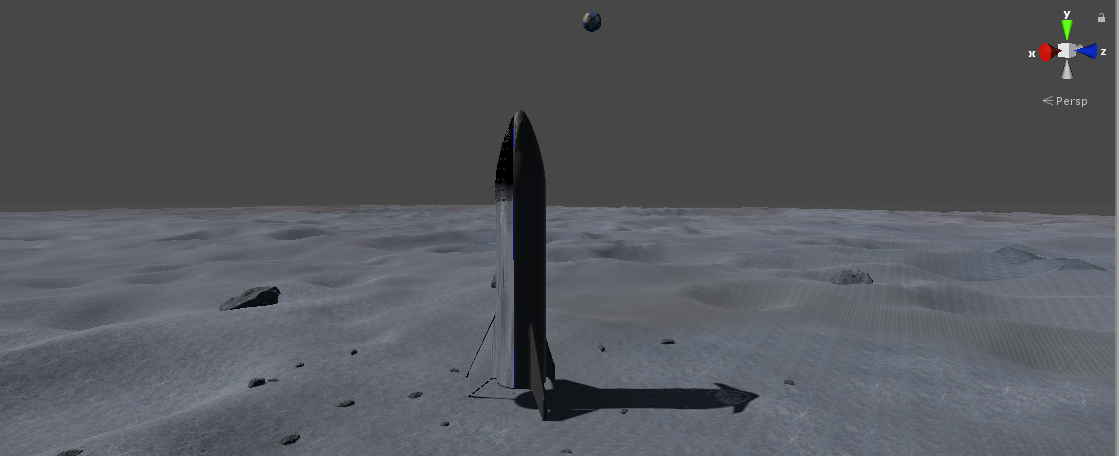
\includegraphics[width=0.85\textwidth]{VirgosRakete.PNG}
\caption{Die Rakete auf der Mondoberfläche}
\end{figure}

Innerhalb der Rakete befindet sich ein Kontrollraum, von dem die Funktionen der Rakete aus gesteuert werden können. Der Kontrollraum verfügt über zwei Türen und zwei Aufzüge, über die man die Rakete verlassen kann. Um die Türen zu öffnen muss zuerst die Luft aus dem Kontrollraum abgelassen werden. Dies geschieht über einen Knopf auf einer Schalttafel. Der Druckabfall wird durch eine Dämpfung der Umgebungsgeräusche simuliert. Anschließend kann eine der beiden Türen über einen anderen Knopf geöffnet werden. Zum Zeitpunkt der Entwicklung war nur eine der Türen und ein Aufzug funktionsfähig. Der Aufzug lässt sich über Knöpfe steuern, die direkt am Aufzug angebracht sind. Über der Schalttafel der Rakete befinden sich drei Bildschirme. Zwei zeigen statische Bilder, während der Dritte eine Endlosschleife eines Videos abspielt. In der Mitte des Kontrollraums befindet sich ein Avatar in Form eines Astronauten, den der Spieler kontrolliert.\newline

\begin{figure}[H]
\centering
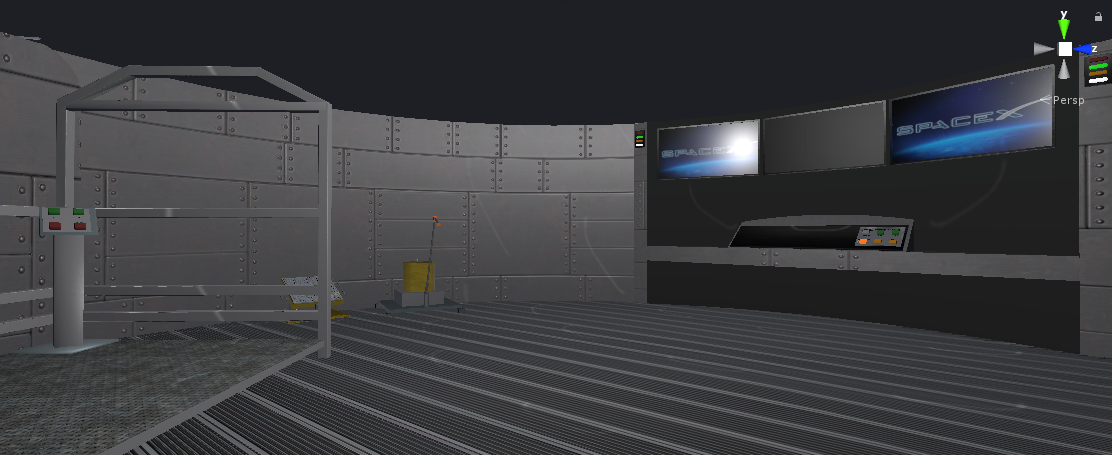
\includegraphics[width=0.85\textwidth]{VirgosKommandozentrale.PNG}
\caption{Der Kontrollraum in der Rakete}
\end{figure}

ViRGOS kann nur von einem Benutzer verwendet werden. Trotzdem verfügt die Anwendung über einen Voice-Chat, der die Kommunikation zwischen dem Benutzer in Virtual Reality und einem Außenstehenden ermöglicht. \\

Die zugehörige Hardware von ViRGOS setzt sich aus einem Virtual Reality Headset, zwei handgehaltenen Controllern, einem Virtualizer und dem Kransystem zusammen. Der Virtualizer ist ein Gerät welches zur Lokomotion in Virtual Reality eingesetzt wird. Es ermöglicht dem Benutzer Bewegungen in alle Richtungen, ohne sich tatsächlich im Raum zu bewegen. Das Kransystem wird verwendet um einen Teil des Körpergewichtes des Benutzers aufzunehmen. Somit kann eine reduzierte Schwerkraft simuliert werden, was zur Immersion in die Weltraum-Umgebung beiträgt. 
 

\section{Stand der Wissenschaft} \label{Wissenschaft}
Dieses Kapitel präsentiert den Stand der Wissenschaft im Bezug auf kooperatives Lernen in Virtual Reality. Zunächst wird auf das Lernen in Virtual Reality allgemein eingegangen und welche Vorteile es zu klassischem Lernen bietet. Anschließend werden Arbeiten behandelt, die sich ebenfalls mit Kooperation in virtuellen Räumen beschäftigen.

\subsection{Lernen in Virtual Reality}
In diesem Kapitel wird sich mit den allgemeinen Möglichkeiten und Vorteilen auseinandergesetzt, die Virtual Reality im Bezug auf den Lernprozess haben kann. Zuerst werden positive Effekte aufgezeigt, die Virtual Reality auf den Lernprozess haben kann. Anschließend wird auf die Theorie der Lerntypen eingegangen, welche dann mit virtuellen Umgebung in Verbindung gebracht werden. Zum Schluss wird eine Theorie der Unterteilung von virtuellen Welten in sogenannte Lernwelten behandelt, welche die Herangehensweise an den Lernprozess, abhängig von dem Ziel der Anwendung, beschreiben.

\subsubsection{Positive Lerneffekte von Virtual Reality}
Virtual Reality bietet viele Vorteile gegenüber klassischen Lernansätzen. Besonders bei praxisorientierten Aufgaben bieten Virtual Reality Anwendungen die Möglichkeit, Bewegungsabläufe nachzuahmen und praktisch anzuwenden. Wenn sich der Lernende rein theoretisches Wissen aneignet ist zusätzlich eine Transferleistung notwendig um dieses Wissen in die Praxis umzusetzen. Zudem ermöglichen diese Anwendungen eine Simulation des Kontextes, in dem das Wissen und die Fähigkeiten des Lernenden gebraucht werden. So kann die spätere Arbeitsumgebung eines Benutzers simuliert werden, wodurch erneut keine Transferleistung von der Trainings- in die Arbeitsumgebung erbracht werden muss.\\

Zusätzlich zu praktischem, kann auch theoretisches Wissen in VR vermittelt werden. Durch das Verknüpfen von theoretischen Informationen mit dem Erlebnis in der 3D-Welt steigert sich das Erinnerungsvermögen der Lernenden. Das räumliche Vorstellungsvermögen verbessert sich durch den Kontakt mit den dreidimensionalen Darstellungen ebenfalls ~\parencite{Buehler2020}.\\

Auch auf wirtschaftlicher Seite bietet VR großes Potential. Wenn größere Gruppen geschult oder unterrichtet werden müssen gibt es das Problem, dass es oft nur begrenztes Trainingspersonal oder Übungsmaterialien gibt. Besonders die Schulung für den Umgang mit größeren Geräten kann problematisch sein, da es zu kostspielig ist ein Übungsgerät für jeden Lernenden bereitzustellen. Wenn sich die Lernenden allerdings mit demselben Gerät abwechseln, erhöht sich die Dauer der Schulung immens. Die Verwendung von VR bietet die Möglichkeit die Lernenden unabhängig von der Gruppe zu schulen. Jeder Benutzer kann hierbei in seinem eigenen Tempo lernen, ohne den Rest der Gruppe auszubremsen oder abzuhängen. Da die Anwendungen so entworfen werden können, dass der Benutzer selbstständig zurecht kommt, muss das Schulungspersonal nur in Ausnahmefällen einschreiten. Somit können Kosten gespart werden, da weniger Personal für größere Gruppen eingesetzt werden muss.\\

Weitere Kosten können gespart werden, da keine Übungsmaschinen angeschafft, oder aus dem laufenden Betrieb entfernt werden müssen. Zudem besteht nicht die Gefahr, dass Benutzer das Übungsgerät falsch verwenden und somit beschädigen. Die Lernenden sind darüber hinaus unabhängig von den Örtlichkeiten. Schulungen können somit überall durchgeführt werden, sofern die notwendige Hardware vorhanden ist. Auch eine Verletzungsgefahr ist so gut wie ausgeschlossen. Somit können Tätigkeiten, die in der Regel gefährlich oder beschwerlich sind, gefahrlos geübt werden ~\parencite{Buehler2020}.

\subsubsection{Lerntypen}
Jeder Lernende hat unterschiedliche Herangehensweisen an den Prozess des Lernens und verschiedene Vorlieben. Trotz der zentralen Wichtigkeit des Lernens im Bezug auf schulische und akademische Leistungen, aber auch darüber hinaus, gibt es viele, teils widersprüchliche Arbeiten, die sich mit der Thematik beschäftigen. Ein weit verbreiteter Ansatz ist das sogenannte VARK-Modell. Hierbei werden vier Gruppen von Lernenden, anhand ihrer bevorzugten Art der Präsentation von Daten, unterschieden:
\begin{itemize}
\item Visuell: Der Lernende bevorzugt es Daten in Form von Bildern, Diagramme usw. zu sehen 
\item Auditiv: Dem Lernenden liegt das Hören oder Aussprechen bzw. Debattieren über Daten am Meisten
\item Lesen/Schreiben: Der Lernende versteht Daten am Besten indem er/sie Texte oder Tabellen liest und Notizen anfertigt
\item Kinästhetisch: Der Lernende wendet gelernte Daten am Liebsten praktisch an um diese zu verinnerlichen
\end{itemize}
Laut dem VARK-Modell können Lernende nicht nur eine Vorliebe für eine dieser Methoden, sondern für mehrere gleichzeitig aufweisen. \\

In einer Studie ~\parencite{8971204} die sich mit der Thematik beschäftigt, wurde festgestellt, dass der Großteil der Lernenden eine Mischung aus allen vier Methoden bevorzugt. Außerdem ist zu dem Schluss gekommen worden, dass Lernende selbst dann keine besseren Lernerfolge vorweisen können, wenn sie exklusiv in ihrer dominanten Lernmethode unterrichtet wurden. Dies verwischt die Grenzen der vier Gruppen und legt eine multimodale Art des Lernens nahe.
Dies wird weiterhin durch Befunde gestützt, die erschließen lassen, dass die Art der Reizverarbeitung ausschlaggebend ist und nicht die Modalität der Reizaufnahme ~\parencite{UBHD-67741817}. Beispielsweise wird Sprache ähnlich verarbeitet wenn sie auditiv oder in geschriebener Form aufgenommen wird. Bilder und Texte hingegen werden visuell wahrgenommen, aber intern unterschiedlich verarbeitet.\\

Basierend auf der Vielzahl von unterschiedlichen Ansätzen ist zu sagen, dass sich sowohl die Präferenzen des Lernen, als auch die Bedingungen der Lernumgebung ausschlaggebend auf den Lernerfolg auswirken ~\parencite{UBHD-67741817}. Virtual Reality stellt durch die potentielle Abdeckung aller Lernmethoden und Sinneskanäle eine vielversprechende Alternative zu klassischem Lernen dar. 

\subsubsection{Interaktion und Lernwelttypen}
Der wohl größte Vorteil, den Virtual Reality im Bezug auf Lernen hat, ist die Möglichkeit der Interaktion mit der virtuellen Welt. Es wurde bereits bestätigt, dass Interaktivität zu einem höheren Engagement bei der Auseinandersetzung mit den Inhalten führt ~\parencite{8864531}. Besonders bei prozeduralem Wissen, also dem Erlernen von Handlungsverläufen, stellte sich die Interaktivität in Virtual Reality als effektives Lehrmittel heraus ~\parencite{8797755}. \newline

Die Art und der Umfang der Interaktivität ist jedoch stark von der Thematik und dem Ziel der Virtual Reality Anwendung abhängig. So können sich virtuelle Lernwelten in 4 verschiedene Gruppen einteilen lassen ~\parencite{UBHD-65563883}:

\begin{itemize}
\item Explorationswelten
\item Trainingswelten
\item Experimentalwelten
\item Konstruktionswelten
\end{itemize}

Ziel der Explorationswelten ist die freie, möglichst uneingeschränkte Begehbarkeit der Welt. So kann beispielsweise eine antike Stadt virtuell nachgebaut und für den Benutzer frei begehbar gemacht werden. Der Benutzer entscheidet hierbei selbst über die Geschwindigkeit und Reihenfolge in der die Elemente der Welt abgearbeitet werden. \\

Bei Trainingswelten steht besonders das Vermitteln von prozeduralen Fertigkeiten im Mittelpunkt. So können Trainingswelten für den Umgang mit Maschinen entwickelt werden. Der Benutzer ist in der Lage sich mit dem Gerät auseinanderzusetzen und die notwendigen Handgriffe zu üben, ohne dass die potentiell teure Maschine tatsächlich angeschafft werden muss. Auch in Situationen die den Lernenden in Gefahr bringen könnten ist vorherige Übung in einer Trainingswelt wie einem Fahrsimulator von Vorteil. \\

Experimentalwelten vermitteln im Gegensatz zu Explorationswelten keine statischen Fakten, sondern versuchen dem Lernenden durch Experimente die geltenden Gesetzmäßigkeiten der virtuellen Welt zu erläutern. Der Benutzer kann zum Beispiel Eigenschaften von Objekten oder der Welt verändern um die Auswirkungen dieser Änderungen zu simulieren und zu verstehen. Experimentalwelten dienen also auch als wissenschaftliches Werkzeug zur Bestätigung oder Wiederlegung eigener Hypothesen. \\

Konstruktionswelten gehen im Vergleich zu Experimentalwelten einen Schritt weiter und verlassen sich mehr auf die Kreativität des Lernenden. In Konstruktionswelten kann der Benutzer die virtuelle Welt selbst nach seinen Vorstellungen oder einer Aufgabenstellung gestalten. Ähnlich wie das bekannte Papierbrücken-Experiment, bei dem Schüler oder Studenten eine möglichst stabile Brücke aus Papier bauen sollen, wird dem Benutzer in einer Konstruktionswelt eine Aufgabe gestellt die umgesetzt werden soll. Mögliche Fehleinschätzungen fallen anhand der laufenden Simulation sofort auf und können angepasst werden. Somit wird sofort aus dem Erfolg oder Misserfolg der eigenen Konstruktion gelernt. Da der Benutzer die Konstruktion selbst durchgeführt hat, zählt hier nicht nur das Endergebnis, sondern auch der Weg, über den zu diesem gelangt wurde. \\

\subsection{Kooperation in Virtual Reality}
In diesem Unterkapitel wird speziell auf die Kooperation in Virtual Reality eingegangen. Zu Beginn wird die Interaktion zwischen mehreren Benutzern thematisiert. Anschließend wird auf die unterschiedlichen Arten der Kommunikation zwischen diesen Benutzern eingegangen. Zum Schluss wird der Sonderfall der asymmetrischen Kooperation sowie die unterschiedlichen Arten der Asymmetrie an mehreren Beispielen erklärt.

\subsubsection{Interaktion mit mehreren Benutzern}
Mit der konstanten Weiterentwicklung der Hardware, als auch der Software von Virtual Reality, erweitern sich auch die Funktionalitäten und Anwendungsbereiche der Technologie. Eine dieser Erweiterungen ist die Anwendung von VR mit mehreren kooperierenden Benutzern. Bereits als die Technologie in den 90er Jahren noch in den Kinderschuhen steckte wurden erste Tests durchgeführt, die das Potential von virtuellen Mehrspieler-Anwendungen beschreiben ~\parencite{youngblut1998educational}.\newline
In der Zwischenzeit fand VR für Kooperation mit mehreren Benutzern einige Anwendungen. Virtual Reality ermöglicht die realistische Darstellung von Objekten aus unterschiedlichen Blickwinkeln. Durch die Darstellung der anderen Benutzer und deren Interaktion mit der virtuellen Umwelt wird eine soziale Erfahrung erzeugt, die Zusammenarbeit und Diskussion über die Thematik ermöglicht ~\parencite{8798289}. Benutzer sind hierbei nicht auf lokale Zusammenarbeit beschränkt, sondern können über große Distanzen kooperieren. Diese Distanz stellt bei Interaktionen in Virtual Reality kein großes Problem dar und kann die Zusammenarbeit sogar erleichtern. Laut einer Studie ~\parencite{8848001} ist die Kooperation in Virtual Reality effektiver wenn die Teilnehmer physikalisch räumlich getrennt sind, statt sich im selben Raum aufzuhalten. 

\subsubsection{Kommunikation}
Ein wichtiger Punkt bei Kooperation in einer virtuellen Umgebung ist die Kommunikation mit anderen Benutzern. Die grundlegende Art der Kommunikation, die von den meisten Anwendungen angeboten wird, ist die gesprochene Sprache über Voice-Chats. Mit anderen Benutzern sprechen zu können ermöglicht bereits den Austausch von vielen Informationen und ist die intuitivste Art der Kommunikation. Gerade in dreidimensionalen Welten verfügt jeder Benutzer über seinen eigenen Blickwinkel auf dasselbe Objekt, wodurch es zu einer Diskrepanz der räumlichen Informationen kommen kann. Ein Benutzer kann verbal auf etwas hinweisen, das ein anderer aufgrund seiner räumlichen Position nicht sehen kann. Jedoch kann die verbale Beschreibung eines Punktes im Raum vage ausfallen, wodurch es den anderen Benutzern schwer fällt zu erkennen was gemeint ist. Eine Möglichkeit dies zu lösen ist die Verwendung von Werkzeugen, die non-verbale Kommunikation erlauben. Bei einer beispielhaften Anwendung\footnote{https://weare-rooms.com/vr-cad/ (Zugriff: 11.05.2020)}, die für die Zusammenarbeit an 3D-Modellen und Dokumenten entworfen wurde, erhält man die Möglichkeit mit seiner virtuellen Hand auf Punkte im Raum zu zeigen. Zusätzlich können Notizen geschrieben und an Objekten platziert werden, um Informationen mehrmals zugänglich zu machen. Außerdem kann auf Objekten gezeichnet werden, um so beispielsweise interessante Punkte zu markieren. Dies sind nur einige der Möglichkeiten, mit denen die Kommunikation mit anderen Benutzern erweitert werden kann.

\subsubsection{Asymmetrische Kooperation}
Eine besondere Unterart der Kooperation in Virtual Reality ist die asymmetrische Kooperation. Asymmetrie bedeutet in diesem Fall, dass es Unterschiede bei der Benutzung der Anwendung gibt. Diese Asymmetrie kann sich hierbei auf unterschiedliche Bereiche beziehen. Zum Beispiel kann es eine Asymmetrie in der Technologie geben, mit der die virtuelle Welt betreten wird. So kann ein Benutzer die Welt mit einem VR-Headset betreten, während ein anderer eine Augmented Reality Technologie oder einen einfachen Desktop-Computer verwendet. Diese Differenz kann Vorteile, aber auch Nachteile in der Kollaboration bringen und ist stark von der Art und dem Ziel der Anwendung abhängig ~\parencite{8798080}. \\

Eine Asymmetrie kann aber auch in Form von unterschiedlichen Perspektiven in derselben Anwendung auftreten. In einer Studie ~\parencite{7563562} wurde eine Anwendung vorgestellt, in der mehrere Benutzer in unterschiedlichen Rollen an einer gemeinsamen Aufgaben arbeiten können. Diese Rollen verfügen über verschiedene Skalierungen der virtuellen Welt, was andere Blickwinkel auf dieselben Objekte ermöglicht. Somit ist ein Benutzer ein Riese, der die komplette Szene von oben herab sieht, während der andere winzig ist und sich zwischen kleinen Objekten in der Szene bewegen kann. Aus beiden Blickwinkeln können Informationen zur Lösung der Aufgabe gesammelt werden, die sich gegenseitig ergänzen. \\

Eine weitere Art der Asymmetrie zeichnet sich durch einen Unterschied in den Funktionalitäten aus, die den Benutzern zur Verfügung stehen. Diese Art der Kooperation kommt besonders häufig bei Lehrer-Schüler-Szenarios zum Einsatz. Die lehrende Person verfügt also über Funktionalitäten oder Werkzeuge, die zum Anleiten des Schülers verwendet werden können. Der Schüler hingegen benötigt keinen Zugriff auf diese Werkzeuge. Ein Beispiel hierfür ist ObserVAR ~\parencite{8943686}, eine Anwendung bei der ein Lehrer mehrere Schüler in Form von Avataren beobachten kann. Dem Lehrer wird hierbei visuell angezeigt auf welchen Punkt im Raum jeder Schüler schaut. Somit kann die Aufmerksamkeit der Schüler gezielt gelenkt werden. Eine weitere Einsatzmöglichkeit ist die Planung eines Raumes. Hier kann sich ein Kunde einen virtuellen Raum vor dem Kauf ansehen. Der Immobilienhändler verfügt nun über die Möglichkeit virtuelle Möbel nach den Vorstellungen des Kunden im Raum zu platzieren ~\parencite{7223433}. \\

All diese unterschiedlichen Arten der Asymmetrie können in verschiedenen Kombinationen auftreten, abhängig von der Art der Kooperation und dem Ziel der Anwendung. In diesem Beispiel der Fernwartung ~\parencite{10.1145/2807442.2807497} kommen sowohl unterschiedliche Technologien als auch Funktionalitäten zum Einsatz. In dieser Anwendung lehrt ein Experte einem anderen Benutzer den Umgang mit einem physikalischen Objekt in Echtzeit. Damit der Benutzer den Anweisungen direkt folgen kann, muss dieser sowohl die Anweisung als auch das physikalische Objekt sehen. Dies wird durch eine Augmented Reality Brille ermöglicht. Der Experte hingegen verwendet eine Virtual Reality Brille und verfügt über Möglichkeiten Markierungen zu setzen und wichtige Informationen an den anderen Benutzer zu übermitteln. 

\section{Konzeption} \label{Konzeption}
In diesem Kapitel werden zu Beginn die an diese Arbeit gestellten Anforderungen behandelt. Diese Anforderungen wurden zu Beginn zusammen mit dem Betreuer des VR-Labors der Hochschule Reutlingen festgelegt. Anschließend wird die Auswahl der Technologien beschrieben, die für dieses Projekt notwendig sind. Im nächsten Unterkapitel werden schließlich die Konzeptionen von sowohl einem Prototypen, als auch der eigentlichen Anwendung erläutert.  

\subsection{Anforderungsanalyse}
Ziel dieser Analyse ist die Identifizierung von sowohl den funktionalen als auch den nicht-funktionalen Anforderungen, die an dieses Projekt gestellt werden. 

\subsubsection{Funktionale Anforderungen}
Basierend auf den an das Projekt gestellte funktionale Anforderungen definieren sich die Funktionen und das Verhalten des Systems.

\subsubsection*{A1 Mehrere Benutzer gleichzeitig in der Anwendung \label{A1}}

Das System soll mehreren Benutzern die gleichzeitige Verwendung ermöglichen.\\

Das System soll: 
\begin{itemize}
\item Mindestens zwei Benutzer gleichzeitig zulassen
\item Dynamisch auf zusätzliche Benutzer reagieren
\end{itemize}

	
\subsubsection*{A2 \label{A2} Keine technische Abhängigkeit von einem VR-Headset}
Das System soll nicht exklusiv über ein Virtual Reality Headset verwendbar sein.\\

Das System soll: 
\begin{itemize}
\item Sowohl über ein VR-Headset als auch einen Desktop-Bildschirm benutzbar sein
\item Sich automatisch auf die jeweilige Hardware einstellen
\end{itemize}

\subsubsection*{A3 \label{A3} Astronaut und Kommandant als Rollen für die Benutzer}
Das System soll die Rollen Astronaut und Kommandant für den Benutzer zur Verfügung stellen.\\

Das System soll: 
\begin{itemize}
\item Die Rollen nicht fest zuweisen
\end{itemize}

Die Benutzer sollen:
\begin{itemize}
\item Die Rollen während der Laufzeit der Anwendung wechseln können
\end{itemize}

\subsubsection*{A4 \label{A4} Informationsübertragung zwischen den Benutzern}
Das System soll dem Kommandanten mehrere Werkzeuge zur Verfügung stellen mit deren Hilfe er mit dem Astronauten kommunizieren kann. \\

Das System soll: 
\begin{itemize}
\item Einen Möglichkeit der sprachlichen Kommunikation anbieten
\item Eine Funktion bieten mit der auf bestimmte Punkte im Raum verwiesen werden kann
\item Eine Funktion bieten mit der die aktuelle Position eines anderen Spielers heraus gefunden werden kann
\item Eine Funktion bieten mit der Notizen an Objekten angebracht werden können
\end{itemize}

Aus diesen ermittelten funktionalen Anforderungen ergibt sich dieses Use-Case-Diagramm:

\begin{figure}[H]
\centering
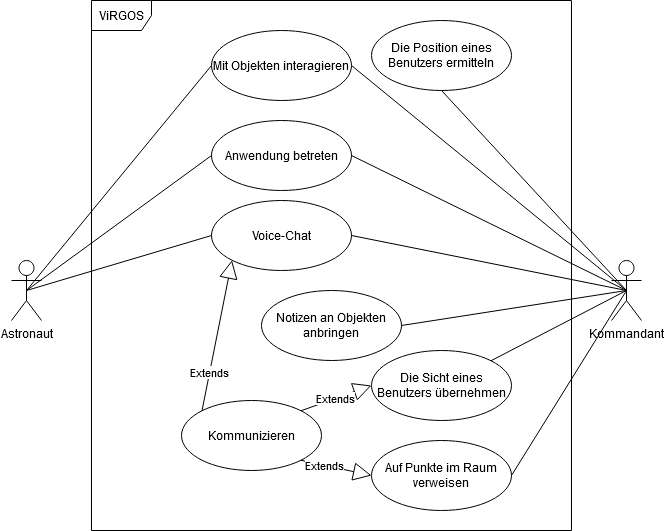
\includegraphics[width=1\textwidth]{ViRGOS_UseCase.png}
\caption{Use-Case-Diagramm von ViRGOS}
\end{figure}

\subsubsection{Nicht-Funktionale Anforderungen}
Die Nicht-Funktionalen Anforderungen geben Charakteristiken an, die in unterschiedlichem Maße in allen Projekten vorkommen.

\subsubsection*{Funktionalität}
Die Funktionen, um welche die Anwendung erweitert wird, sollen zum Erreichen des Ziels dieser Arbeit beitragen. Durch die experimentelle Natur dieser Thesis müssen die implementierten Funktionalitäten nicht final sein, sondern können in der Zukunft erweitert oder angepasst werden. Da zu jedem Zeitpunkt mehrere Studierende an unterschiedlichen Teilen dieses Projekts arbeiten, müssen spätestens bei der Zusammenführung Anpassungen vorgenommen werden.

\subsubsection*{Zuverlässigkeit}
Da das Ziel der Anwendung die Kooperation von mehreren Benutzern ist, muss jede Interaktion mit Objekten zuverlässig über alle Instanzen synchronisiert werden. Wenn ein Benutzer einen Knopf drückt um zum Beispiel eine Tür zu öffnen, und sich diese bei einem anderen Benutzer nicht auch öffnet, kommt es zu einer Diskrepanz in der Spielwelt. Dies kann zu einer Erschwerung in der Kommunikation führen, wenn Unsicherheit darüber besteht ob alle Benutzer exakt dasselbe sehen. Die Fehlertoleranz der Anwendung kann im Falle der Synchronisation von Positionen etwas höher sein, da diese Informationen mehrmals pro Sekunde abgeglichen werden. Bei einmaligen Benutzungen von Werkzeugen muss dies allerdings geringer ausfallen.
Da in der Anwendung keine Daten gespeichert werden gibt es keinen Grund einen Fokus auf Wiederherstellbarkeit im Fehlerfall zu setzen. Auch im Bezug auf Verfügbarkeit gibt es große Toleranzen da die Anwendung, aufgrund der notwendigen Einrichtung der Hardware, nur unregelmäßig verwendet wird.

\subsubsection*{Gebrauchstauglichkeit}
Da die Anwendung primär von Experten der Materie benutzt wird, und alle Laien von Experten begleitet werden, muss die Anwendung nicht zwingend einfach zu erlernen sein. Es sollte keine große Anfälligkeit für Fehler von Seiten der Benutzer geben, da sie nur eine begrenzte Menge an Funktionen zur Verfügung haben und die Experten des Labors einer falschen Benutzung vorbeugen. Da es sich bei dieser Arbeit um eine Virtual Reality Anwendung handelt, gibt keine Anforderungen an das Benuter-Interface, da die Anwendung optimalerweise gänzlich ohne ein Interface auskommt. 

\subsubsection*{Sicherheit}
Sicherheit ist bei diesem Projekt keine große Priorität, da die Anwendung exklusiv von Mitgliedern des Virtual Reality Labors benutzt wird. Somit haben Außenstehende keinen Zugriff auf die Soft- oder Hardware, weshalb zusätzliche Maßnahmen zur Stärkung der Sicherheit nicht notwendig sind.

\subsubsection*{Effizienz}
Die Anwendung muss Änderungen sehr schnell über alle Instanzen synchronisieren um eine Immersion der Benutzer zu gewährleisten. Durch zu große zeitliche Abweichungen in der Datenübertragung kann es zu Asymmetrien in den Instanzen kommen, was die Zusammenarbeit erschweren kann. Des Weiteren muss die Anwendung genügend Kapazitäten für die Benutzer anbieten. Da das Ziel dieser Arbeit nur zwei Benutzer gleichzeitig vorsieht, halten sich die notwendigen Kapazitäten relativ niedrig. 

\subsubsection*{Wartbarkeit}
Da das Projekt auf der Arbeit von anderen Kommilitonen basiert und in Zukunft eventuell weiterentwickelt und erweitert werden soll, ist die Erweiterbarkeit eine wichtige Anforderung. Auch für abgewandelte Tests die in Zukunft durchgeführt werden könnten ist beispielsweise eine dynamische Anpassung an unterschiedliche Spielerzahlen unumgänglich.

\subsubsection*{Portabilität}
Da die Anwendung von spezieller Hardware, namentlich einem Virtual Reality Headset und einem Virtualizer, abhängt, gibt es keine große Anforderungen an die Portabilität. Die Software wird voraussichtlich nur im Rahmen des Virtual Reality Labors verwendet, und muss selten auf anderer Hardware installiert werden.

\subsubsection*{Kompatibilität}
ViRGOS interagiert ausschließlich mit anderen Instanzen von sich selbst. Somit muss die Anwendung mit keinem anderen Programm kompatibel sein. Es muss allerdings eine Koexistenz mit der Treibersoftware, die die notwendige Hardware kontrolliert, möglich sein. 


\subsection{Auswahl der Technologien}
Aufgrund der Tatsache dass ViRGOS in Unity entwickelt wurde und als Basis für diese Arbeit dient, wird Unity auch hier als Entwicklungsumgebung verwendet. Um die Mehrspieler-Funktionalitäten umzusetzen, wurden die Möglichkeiten von UNet, Unitys eigener Mehrspieler-Lösung, geprüft. Unglücklicherweise ist UNet überholt und soll in naher Zukunft entfernt werden. Somit musste sich für eine Framework-Alternative entschieden werden.

\subsubsection{Mirror}
Eine mögliche Lösung stellte Mirror dar. Dieses Framework ist für große Spielerzahlen ausgelegt, die in ViRGOS nicht vorkommen werden. Zudem bietet Mirror eine große Menge an Werkzeugen für die Netzwerk-Entwicklung, ist aber dadurch nicht so anfängerfreundlich wie die Alternative. Die Architektur von Mirror sieht die Entwicklung eines Servers vor, der die Anwendung für die einzelnen Clients hostet. Da dies zusätzlichen Aufwand und Ressourcen benötigen würde, ist Mirror nicht optimal für dieses Projekt geeignet. 

\subsubsection{Photon}
Eine weitere Option ist Photon. In diesem Framework wird die Anwendung auf einem Cloud-Server gehostet, was den Zugriff von überall ermöglicht und die Verbindung zwischen Clients vereinfacht. Zudem ist das Framework weit verbreitet was eine große Wissensgrundlage und Hilfestellungen bietet. Des Weiteren bietet Photon eine kostenlose Version, die nur in der Größe der Cloud Server eingeschränkt ist, aber sonst alles bietet was für die Umsetzung dieses Projektes gebraucht wird. Somit wurde Photon für die Umsetzung gewählt. 

\subsection{Entwurf}
Das Kapitel des Entwurfs beschreibt die Entwicklung der Konzepte von sowohl eines Prototypen als auch der eigentlichen Funktionalitäten in ViRGOS. Die Entwürfe bezüglich ViRGOS sind in die Mehrspielerfähigkeit der Anwendung im Allgemeinen und die Werkzeuge für die Kooperation gegliedert. Abschließend wird ein Entwurf für Tests der Anwendung und eine Befragung von Probanden im Rahmen einer Studie vorgestellt.

\subsubsection{Prototyp}
Um sich mit Unity und Photon vertraut zu machen soll anfangs ein Prototyp entwickelt werden. Hier soll getestet werden wie mit Photon eine Lobby für mehrere Spielern erstellt werden kann. Anschließend sollen einfache Interaktionen mit Objekten implementiert werden. Wenn mehrere Benutzer die Anwendung gleichzeitig verwenden und mit Objekten interagieren können, soll getestet werden wie mit Kollisionen umgegangen werden kann. Hierbei sind Kollisionen mehrerer Interaktionen gemeint, also mehrere Benutzer die gleichzeitig versuchen auf ein Objekt zuzugreifen. Zudem soll die Synchronisation von Zuständen getestet werden. Wenn ein Benutzer mit einem Objekt interagiert und dieses Objekt beispielsweise seine Position ändert, muss dies auch bei allen anderen Benutzern passieren. 


\subsubsection{Mehrspielerfähigkeit in ViRGOS}
Zu Beginn soll ViRGOS um Photon erweitert werden, um mehreren Benutzern den gleichzeitigen Zugriff auf die Anwendung zu ermöglichen. Die Avatare sollen instanziiert werden sobald ein Benutzer beitritt. Somit ist die Anzahl der Benutzer dynamisch und muss nicht im Voraus festgelegt werden. Die Anwendung ist zwar für zwei Benutzer ausgelegt, kann aber in Zukunft weiterentwickelt werden. Somit sollte die Option von mehr als zwei Benutzern offen gehalten werden. Um eine Anweisung des Astronauten durch den Kommandanten notwendig zu machen soll eine Aufgabe für den Astronauten implementiert werden. Diese Aufgabe soll komplex genug sein, dass eine Anweisung über den Voice-Chat nicht immer ausreicht. Um die Verwendung von weiteren Werkzeugen notwendig zu machen, soll sich der Aufbau, der die Aufgabe darstellt, außerhalb der Rakete befinden. 

\subsubsection{Werkzeuge}
Um die aktuelle Position des Astronauten zu ermitteln, soll der Kommandant die Möglichkeit haben sich das Sichtfeld des Astronauten auf einem der Bildschirme anzeigen zu lassen. Somit weiß der Kommandant vor welchem Problem sich der Astronaut gerade befindet. Da die Bildschirme der Kommandozentrale relativ hoch platziert und nicht sehr groß sind, reichen diese nicht aus um kleine Details wahrzunehmen. Ein weiteres Werkzeug das dem Kommandanten zur Verfügung stehen soll, ist die Möglichkeit sein eigenes Sichtfeld durch das des Astronauten zu ersetzen. Somit wird nicht nur auf einem kleinen Bildschirm dargestellt was der Astronaut sieht, sondern es wird möglich durch die Augen des Astronauten zu sehen. Somit verfügt der Kommandant über dieselben Informationen wie der Astronaut, ohne dass dieser alles über den Voice-Chat schildern muss. \\

\noindent Um Informationen an den Astronauten zu übermitteln sollen dem Kommandanten neben dem Voice-Chat verschiedene Werkzeuge zur Verfügung stehen. Es soll ein Zeiger-Werkzeug implementiert werden, dass es ermöglicht auch aus einiger Entfernung auf einen bestimmten Punkt zu verweisen. Somit können präzise Anweisungen an den Astronauten übermittelt werden. Um dies auch dann zu ermöglichen wenn sich beide Nutzer nicht in nächster Nähe befinden, soll sich das Zeiger-Werkzeug auch verwenden lassen, wenn der Kommandant den Bildschirm verwendet und das Sichtfeld des Astronauten verwendet. Dies ermöglicht dem Kommandanten auf einen bestimmten Punkt im Sichtfeld des Astronauten hinzuweisen. \newline

Ein weiteres Werkzeug zur Übermittlung von Informationen an den Astronauten ist die Möglichkeit Notizen zu erstellen und zu platzieren. Der Kommandant soll eine neue Notiz anlegen und diese über eine Virtual Reality Tastatur mit Text befüllen können. Diese fertige Notiz soll dann für den Astronauten sichtbar an Objekten platziert werden können. Somit können wichtige Informationen mit Bezug auf ein Objekt in der Szene auf Abruf an den Astronauten übermittelt werden. Dies kann besonders für schwer zu merkende Informationen nützlich sein die mehrmals gebraucht werden. 

\subsubsection{Tests und Befragungen}
Bereits während der Entwicklung an ViRGOS sollen Tests mit Probanden durchgeführt werden. Diese Personen sollen unterschiedliche Mengen an Erfahrungen mit Virtual Reality Anwendungen haben. Die Tests sollen Aufschluss darüber geben, ob die implementierten Funktionen intuitiv zu benutzen sind oder weiterer Anpassung bedürfen. 

Nach Abschluss der Entwicklung soll eine Befragung mit mehreren Teilnehmern durchgeführt werden. Die Teilnehmer sollen mit einem Virtual Reality Headset, in der Rolle des Astronauten, die Anwendung betreten. Unter Anleitung des Kommandanten sollen sie die Rakete über den Aufzug verlassen und sich zu dem Testaufbau begeben. Dort angekommen sollen sie die Aufgabe durchführen. Um die Unterschiede der Werkzeuge zu testen, sollen die Tests unterschiedlich ablaufen.

\begin{itemize}
\item[Test 1]  Der Astronaut soll nur über den Voice-Chat und ohne den Bildschirm angeleitet werden
\item[Test 2]  Der Astronaut soll nur über den Voice-Chat mit dem Bildschirm angeleitet werden
\item[Test 3]  Der Astronaut soll nur mit dem Zeiger-Werkzeug und dem Notizen-Werkzeug über den Bildschirm angeleitet werden
\item[Test 4]  Der Astronaut soll über den Voice-Chat UND mit den Werkzeugen angewiesen werden
\end{itemize}

Anschließend sollen die Probanden Fragen beantworten, die Auskunft über die Effektivität der unterschiedlichen Unterweisungen geben. Jeder Proband soll alle Tests durchlaufen. Somit kann jeder Proband die Unterschiede zwischen den Methoden und eventuell die eigenen Präferenzen schildern. Die Reihenfolge der Tests soll bei jedem Probanden rotieren. Somit kann eine Befangenheit des Probanden verhindert werden, was zu ungenauen Ergebnissen bei den späteren Tests führen kann. \newline

Diese Chance soll zudem genutzt werden, um das Basissystem ViRGOS zu evaluieren. Die Benutzer sollen die Benutzbarkeit der Anwendung und den Grad der Immersion im allgemeinen bewerten. Außerdem sollen sowohl das Kransystem als auch der Virtualizer von den Benutzern bewertet werden. 

Eine weitere Erkenntnis die aus diesen Tests gewonnen werden kann sind potentielle Unterschiede in der Immersion des Kommandanten. Die Hälfte der Tests soll durchgeführt werden während der Kommandant ein Virtual Reality Headset trägt. Bei der anderen Hälfte befindet sich der Kommandant an einem Computer und steuert seinen Avatar über die Maus und Tastatur. Ihm stehen in beiden Fällen sämtliche Werkzeuge zur Verfügung. Hiermit soll ermittelt werden ob eine Immersion des Kommandanten während der Anleitung des Astronauten vorteilhaft ist. Der hierzu entwickelte Fragebogen befindet sich im Anhang dieser Arbeit.

\section{Umsetzung} \label{Umsetzung}
Zu Beginn wird in diesem Kapitel die Umsetzung des Prototyps beschrieben, welcher zu Testzwecken entwickelt wurde. Anschließend wird die Entwicklung der Funktionalitäten erklärt, um die ViRGOS erweitert wurde. Als Letztes werden Einschränkungen genannt, die sich aufgrund der Covid-19-Pandemie auf die Arbeit ausgewirkt haben.

\subsection{Vorstudie und Prototyp} \label{Vorstudie}
Zu Beginn der Arbeit wurde ein Prototyp entwickelt um sich mit Unity und dem Photon-Plugin auseinanderzusetzen. Außerdem konnten so Funktionalitäten schnell und einfach getestet werden bevor sie in ViRGOS umgesetzt wurden. Der Prototyp ist nicht auf Virtual Reality ausgelegt und diente rein als Testumgebung. Anfangs bestand der Prototyp aus einem einfachen Raum mit vier Wänden und einem Tisch, auf dem eine hölzerne Kiste steht. Diese Kiste kann geöffnet und geschlossen werden, indem diese mit der Maus angeklickt wird. Im Raum befindet sich außerdem ein Avatar, über den der Spieler die Kontrolle übernimmt sobald er das Spiel startet. Der Tisch wurde aufgrund seiner Einfachheit selbst modelliert. Sowohl die Kiste als auch der Avatar hingegen stammen aus dem Unity Asset Store, um Arbeit bei der Modellierung zu sparen, da der Fokus des Prototyps auf den technischen Funktionalitäten liegt. Der Avatar verfügt über ein C\# Skript das dem Spieler ermöglicht diesen zu Bewegen und sich mit der Maus umzusehen.\\

\begin{figure}[H]
\centering
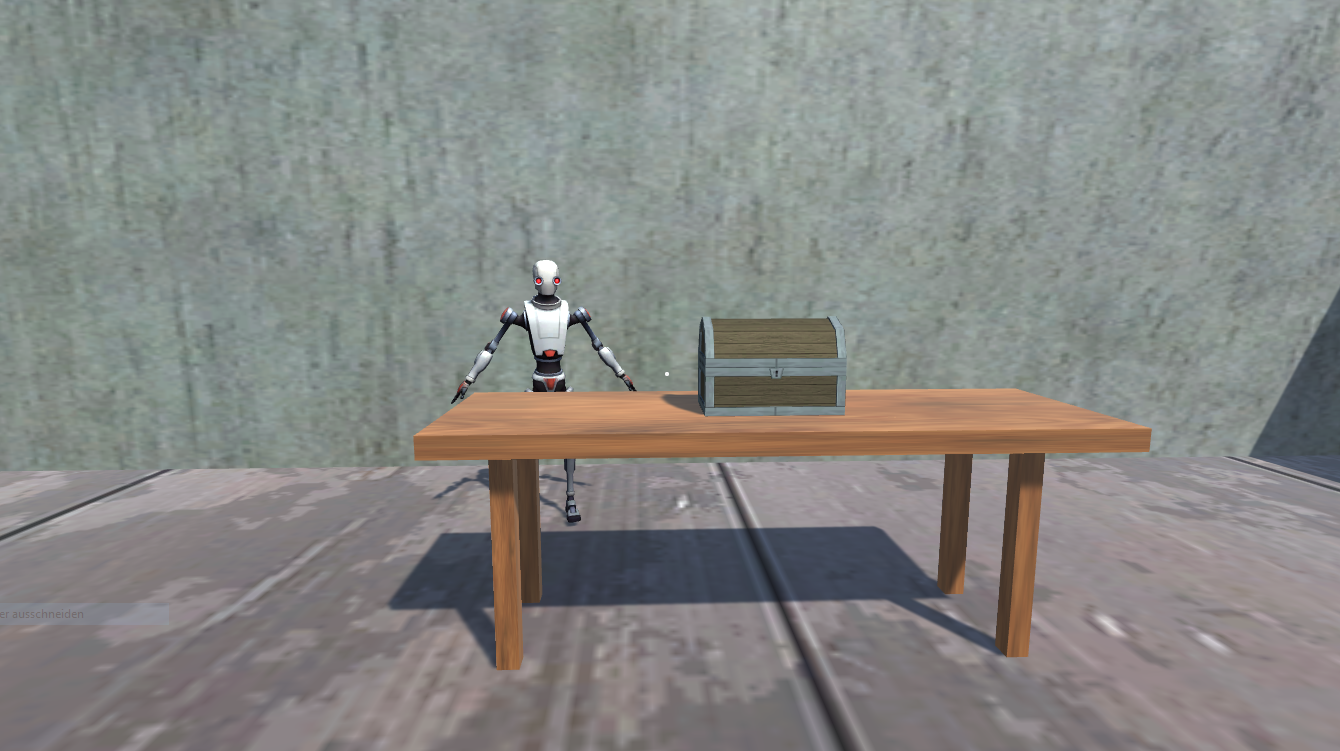
\includegraphics[width=0.75\textwidth]{InteractivityPrototype.PNG}
\caption{Ein Avatar des Prototyps}
\end{figure}

Um mehreren Spielern gleichzeitigen Zugriff auf die Anwendung zu geben, wird das PUN-Plugin von Photon verwendet. Über C\# Skripte werden sowohl die Verbindung zu dem Photon-Server hergestellt, als auch eine Lobby und ein Raum erstellt ~\parencite{InfoGamer2018}.
Hierbei muss nun beachtet werden, dass der Avatar nicht mehr im Voraus in der Szene platziert sein darf. Der erste Spieler kann diesen zwar kontrollieren, aber der zweite Spieler überschreibt die Kontrolle über den Avatar sobald er beitritt. Um dieses Problem zu lösen, werden die Avatare der Spieler über ein Skript dynamisch der Szene hinzugefügt, sobald diese beitreten. Somit muss die Anzahl der Spieler nicht im Voraus festgelegt werden. Um das neue Problem zu lösen, dass sich während des Beitritts keine verfügbare Kamera in der Szene befindet, wird eine zweite Szene in Form eines Menüs verwendet. Jeder Spieler der beitreten möchte befindet sich solange in diesem Menü, bis in der Hauptszene ein Avatar fertig vorbereitet ist, und wird dann in diese weitergeleitet. \newline

Alle Objekte, die mehrfach instanziiert werden und über das Netzwerk identifiziert werden sollen, erhielten eine sogenannte PhotonView-Komponente. Die Skripte, die für die Bewegungen des Avatars und der Kamera zuständig sind, beziehen sich bei einer Mehrspieler-Anwendung auf die lokale PhotonView-Komponente um zu verhindern dass sich alle Instanzen bewegen. Ohne diese Vorkehrung könnte ein Benutzer alle Avatare in der Anwendung steuern. \\

Um die Interaktionen der Spieler mit ihrer Umgebung über alle Instanzen zu synchronisieren, wurde ein Remote Procedure Call (RPC) verwendet. Diese RPCs erlauben es Methoden von anderen Objekten im Netzwerk aufzurufen. In diesem Fall wurde hiermit das Öffnen und Schließen der Kiste synchronisiert. Wenn ein Benutzer auf die Kiste klickt, wird die RPC Methode jeder Instanz des Objektes aufgerufen, welche den Zustand der Kiste von geschlossen zu geöffnet ändert, und anders herum. Dies bedeutet dass die Kisten bei allen Benutzern, inklusive der Eigenen, ihren Zustand ändern, sobald ein Benutzer mit seiner Kiste interagiert. Dies erzeugt den Eindruck dass sich alle Benutzer im selben Raum befinden und mit der gleichen Kiste interagieren. Eine Sperrung der Kiste, um Kollisionen in der Interaktion zu verhindern, war in diesem Fall nicht notwendig. Sollte ein Benutzer mit der Kiste interagieren während die Animation noch nicht abgeschlossen ist, wird die Animation abgebrochen und aus der aktuellen Position in die andere Richtung fortgesetzt. Wenn also mit einer sich schließenden Kiste interagiert wird bevor diese komplett geschlossen ist, wird nahtlos die Öffnungs-Animation aus der aktuellen Position ausgeführt. \newline 
Eine Möglichkeit die Interaktion mit Objekten zu erleichtern ist eine Highlight-Funktion, welche in diesem Prototypen getestet wurde. Wenn ein Benutzer mit dem Cursor auf ein Objekt zielt mit dem interagiert werden kann, wird dieses farblich gekennzeichnet. Dies erleichtert es dem Benutzer zwischen dekorativen und interaktiven Objekten zu unterscheiden.

\subsection{ViRGOS}
In diesem Unterkapitel wird die Umsetzung der Funktionalitäten in ViRGOS thematisiert. Zu Beginn wird geschildert wie die Anwendung erweitert wurde, sodass diese mehrere Spieler gleichzeitig zulässt. Anschließend wird erklärt wie der für den Astronauten gedachten Versuchsaufbau implementiert wurde. Zum Abschluss wird auf die Werkzeuge eingegangen die für die Kommunikation zwischen den Benutzern zuständig sind. 

\subsubsection{Mehrspielerfähigkeit}
Um ViRGOS mit mehreren Spielern zu benutzen wurden dieselben Schritte durchgeführt, die zuvor in Kapitel \ref{Vorstudie} getestet wurden. Nachdem das Photon-Plugin in das Projekt eingebunden war wurden Skripte erstellt die einen Raum und eine Lobby erzeugen. Auch hier wurde der Avatar aus der Szene entfernt, um ihn dynamisch zu instanziieren sobald ein Benutzer beitritt. Zusätzlich zu der PhotonView, die für die Referenzierung über das Netzwerk notwendig ist, wurde der Avatar mit einer Photon Transform View ausgestattet, die die Position und die Rotation der Avatare über alle Instanzen der Anwendung synchronisiert.

\begin{figure}[H]
\centering
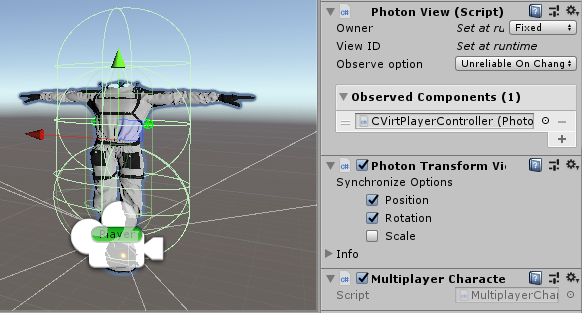
\includegraphics[width=0.75\textwidth]{UnityComponents.PNG}
\caption{Der Avatar mit Photons Multiplayer-Komponenten}
\end{figure}

Ebenso wurde eine Menü-Szene erstellt, die der Haupt-Szene Zeit gibt eine Instanz des Avatars zu erschaffen. Wie in dem Prototyp musste auch hier darauf geachtet werden, dass der Spieler nur seinen eigenen Avatar kontrollieren kann. Wenn ein Spieler beitritt, wird geprüft ob ein Avatar eine lokale Instanz ist oder nicht. Dies wird über die PhotonView Komponente erreicht. Wenn ein Avatar eine lokale Instanz ist, wird dieser von dem am Gerät befindlichen Benutzer gesteuert. Die Skripte, die für die Bewegung des Avatars zuständig sind, werden bei allen Instanzen deaktiviert die nicht lokal sind. Somit kann ein Benutzer nur seinen eigenen Avatar kontrollieren.\\

Um die bereits existierenden Funktionen der Rakete und Aufzüge über das Netzwerk zu synchronisieren, wurden diese so angepasst, dass sie zentralisiert verarbeitet werden. Alle Funktionen der Rakete werden von einem zentralen Skript entgegengenommen. Auch die Funktionen der Aufzüge werden zentralisiert abgearbeitet. In diesen zentralen Skripten werden RPCs angewandt, um diese Aufrufe über die Instanzen zu synchronisieren. Betätigt ein Benutzer nun einen Knopf, um beispielsweise eine Tür der Rakete zu öffnen, sendet das zentralisierte Skript einen RPC an alle Instanzen mit der Bezeichnung des betätigten Knopfes. Somit führen alle Instanzen die jeweilige Funktion aus die dem Knopf zugeordnet ist, was dazu führt, dass sich bei jedem Spieler die Tür der Rakete öffnet.

\begin{figure}[H]
\centering
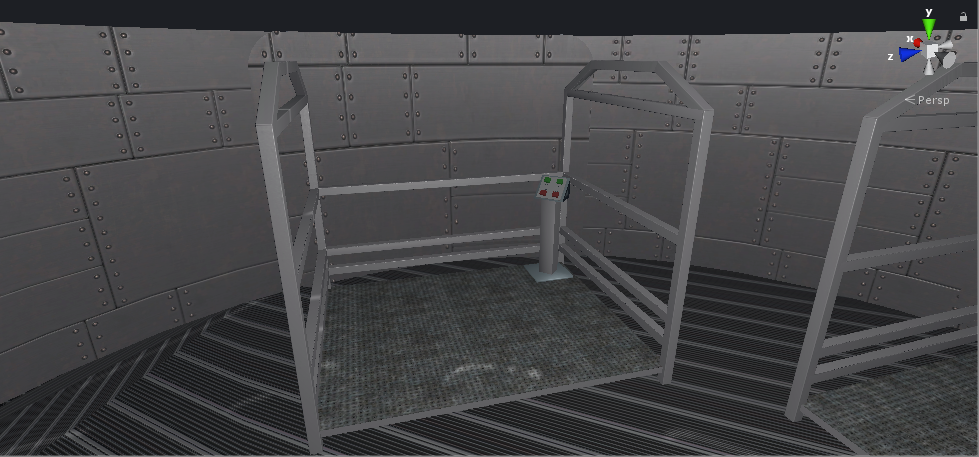
\includegraphics[width=0.75\textwidth]{Elevator.PNG}
\caption{Einer der Aufzüge mit dem zugehörigen Steuerpult}
\end{figure}

Um die Kollision von Interaktionen mehrerer Benutzer zu verhindern, wurde eine Stoppuhr in das Skript der zentralen Raketensteuerung implementiert. Diese Stoppuhr beginnt zu laufen, sobald ein Knopf in der Szene betätigt wird. Das zentrale Kontrollskript blockiert nun die Annahme von sämtlichen Signalen von Knöpfen für eine Sekunde. Dies verhindert, dass ein Knopf aus Versehen zu lange gedrückt wird, was von dem Programm als erneutes Drücken interpretiert werden kann. Außerdem wird so das Problem der Kollision von Interaktionen gelöst. Falls zwei Benutzer denselben Knopf zur gleichen Zeit drücken wollen wird nur die erste Aktivierung angenommen, da der Knopf anschließend für eine Sekunde gesperrt ist.

\begin{figure}[H]
\centering
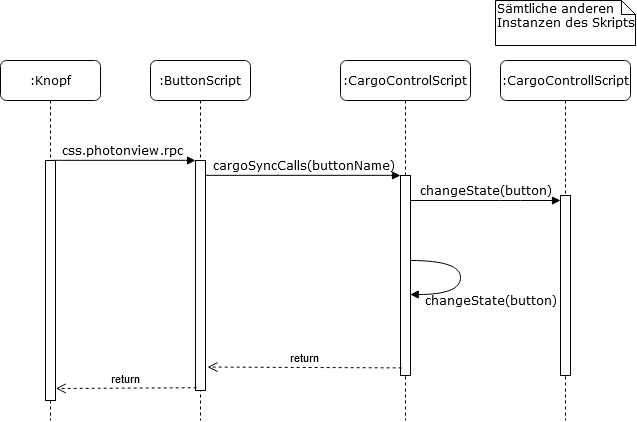
\includegraphics[width=1\textwidth]{RPC.PNG}
\caption{Sequenzdiagramm der RPCs}
\end{figure}

\subsubsection{Versuchsaufbau für Interaktionen} \label{Versuchsaufbau}
Um die Interaktionen zwischen mehreren Benutzern testen zu können, musste zuerst eine Aufgabe entwickelt werden die die Benutzer lösen können. Da der Kommandant, wie im Kapitel \ref{Problemstellung} erklärt, den Astronauten anleiten soll, wurde sich für eine Problemstellung außerhalb der Rakete entschieden. Somit kann der Kommandant in dem Kontrollraum bleiben und den Astronauten unterstützen, während dieser einer Aufgabe nachgeht.

\begin{figure}[H]
\centering
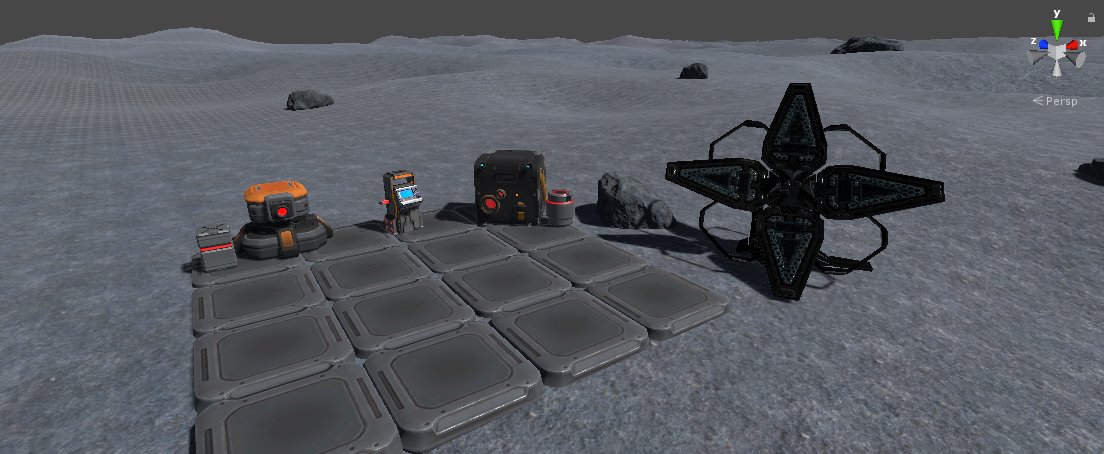
\includegraphics[width=1\textwidth]{InteraktionStation.PNG}
\caption{Der Versuchsaufbau außerhalb der Rakete}
\end{figure}

\subsubsection*{Erste Iteration}
In der ersten Iteration der interaktiven Aufgabe kamen Objekte aus dem Unity Asset Store zum Einsatz. Es wurde aus Gründen der Immersion darauf geachtet, dass diese zu der Weltraumthematik passen. Speziell ein futuristischer Geldautomat, ein Geschützturm, das Modell einer Drohne und eine Satellitenschüssel wurden ausgewählt, unter anderem weil diese kostenfrei verfügbar waren. 

\begin{figure}[H]
\centering
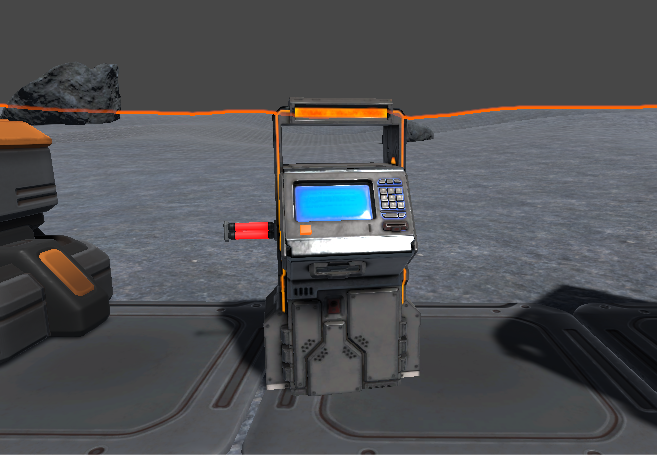
\includegraphics[width=0.8\textwidth]{ATM.PNG}
\caption{Das Modell des Geldautomaten}
\label{fig:ATM}
\end{figure}

Sowohl der Geschützturm als auch die Satellitenschüssel sowie der Geldautomat verfügen über keinerlei eigene Funktionen. Das Modell der Drohne verfügt über bewegliche Teile, die alle eigene Animationen besitzen. Zusätzlich wurde eine Sammlung von Fässern in verschiedenen Designs verwendet, einerseits um die Szene etwas mehr auszufüllen, andererseits um sie als Indikatoren zu verwenden. Jedes dieser Fässer besitzt eine leuchtende, farbige Komponente. Indem die Größe und Position der Fässer angepasst wird, können diese von den Spielern als Signallampe der interaktiven Objekte wahrgenommen werden. In Abbildung \ref{fig:ATM} ist das Modell des Geldautomaten zu sehen. An der linken Seite des Modells, befindet sich ein kleines, rotes Objekt. Dieses Objekt ist eines der Fässer, welches in diesem Fall als Indikator eingesetzt wird. 

\begin{figure}[H]
\centering
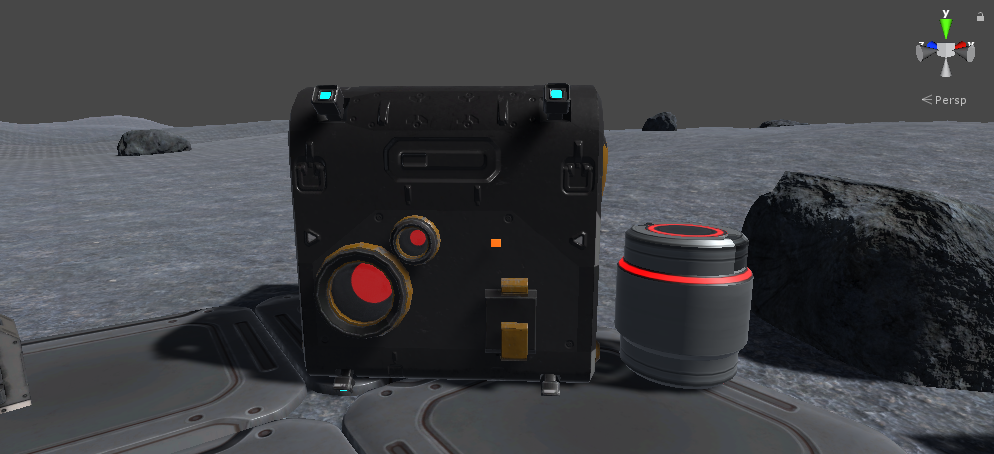
\includegraphics[width=0.8\textwidth]{Drone.PNG}
\caption{Das Modell der Drohne}
\end{figure}

Jede der interaktiven Maschinen wurde mit einem Knopf ausgestattet, der die Farbe der Fässer in unmittelbarer Nähe zwischen rot und grün wechselt. Dies soll den Eindruck erwecken, dass die Maschine an- oder ausgeschaltet ist. Das Modell der Drohne spielt zusätzlich die Animationen aller Einzelteile ab. Wenn alle Maschinen gleichzeitig angeschaltet sind, wechselt die Satellitenschüssel ihre Farbe von schwarz zu grün. Damit ist die Aufgabe für den Spieler abgeschlossen.\newline

\begin{figure}[H]
\centering
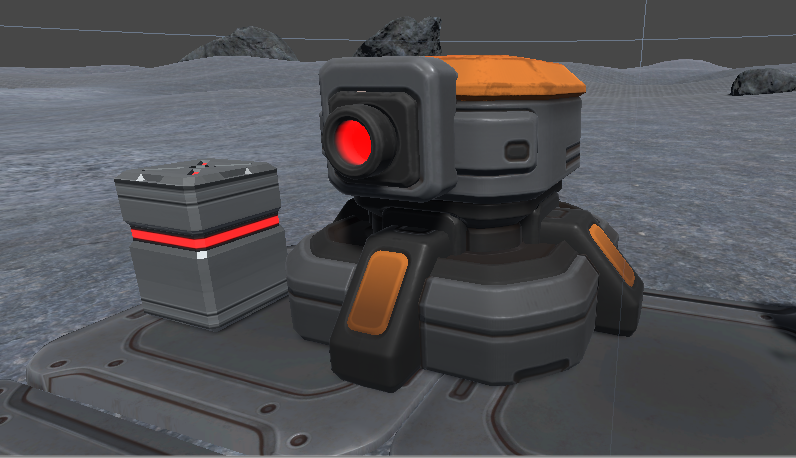
\includegraphics[width=0.8\textwidth]{Turret.PNG}
\caption{Das Modell des Geschützes}
\end{figure}

\begin{figure}[H]
\centering
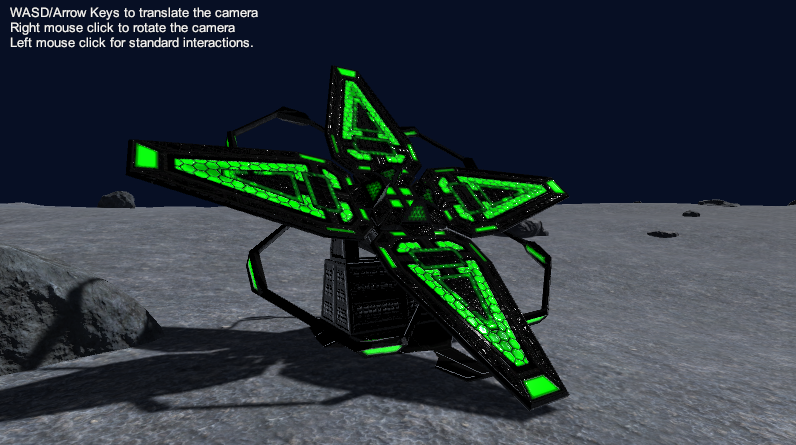
\includegraphics[width=0.8\textwidth]{SatelliteDish.PNG}
\caption{Die Satellitenschüssel in angeschaltetem Zustand}
\end{figure}

\subsubsection*{Zweite Iteration}
Um die Wahrscheinlichkeit zu erhöhen, dass der Astronaut Unterstützung bei der Lösung der Aufgabe benötigt, wurde der Versuchsaufbau weiterentwickelt. Die einzelnen Bauteile der Drohne verfügen bereits von Haus aus über Animationen, die die Objekte allerdings automatisch in die Ausgangsposition zurück bewegen. 

\begin{figure}[H]
\centering
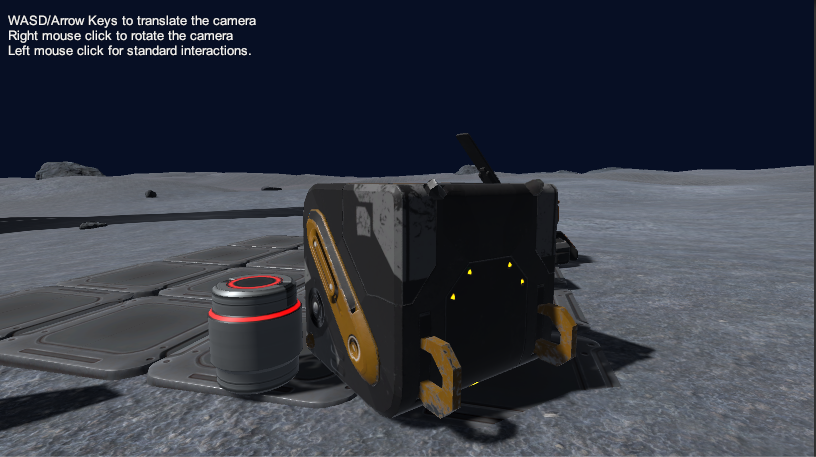
\includegraphics[width=0.8\textwidth]{DrohneGeschlossen.PNG}
\caption{Die Rückseite der Drohne in geschlossenem Zustand}
\end{figure}

Um dies zu verhindern wurden alle Animationen auf die Hälfte gekürzt. Die Einzelteile der Drohne bleiben somit in ihrer ausgefahrenen Position stehen, wodurch die Benutzer Zugriff auf den Innenraum der Drohne erhalten. Ein weiterer Druck auf den Knopf spielt die Animation nun rückwärts ab, und alle Einzelteile bewegen sich in ihre Ausgangsposition. Dies ermöglicht eine komplexere Aufgabenstellung, indem weitere Knöpfe im Inneren des Geräts versteckt wurden. Um die Drohne zu aktivieren, muss der Astronaut die Drohne öffnen, alle drei Knöpfe im Inneren aktivieren und diese wieder schließen.

\begin{figure}[H]
\centering
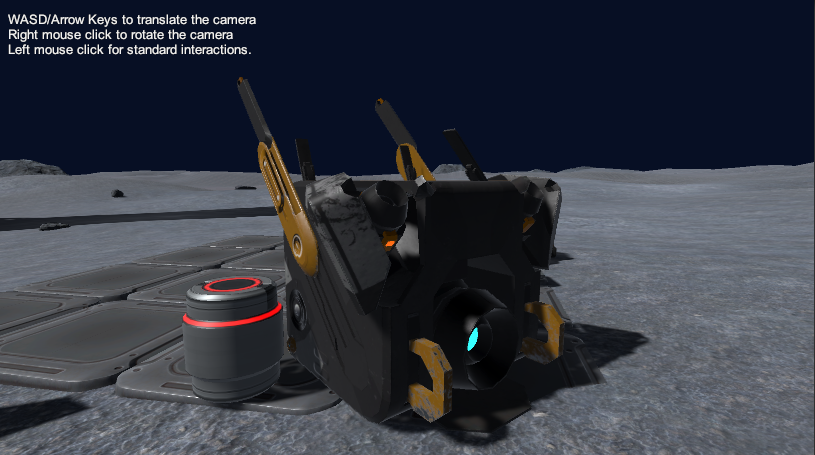
\includegraphics[width=0.8\textwidth]{DrohneOffen.PNG}
\caption{Die Rückseite der Drohne in geöffnetem Zustand}
\end{figure}

\subsubsection{Werkzeuge}
Damit der Kommandant den Astronauten anleiten kann muss dieser wissen, woran der Astronaut aktuell arbeitet. Da sich der Astronaut außerhalb der Rakete befindet, hat der Kommandant keinen direkten Blickkontakt zu ihm. ViRGOS war zu Beginn dieser Arbeit bereits mit einer Voice-Chat Funktion ausgestattet, was die Kommunikation ermöglicht. Die Anwendung wurde durch eine visuelle Komponente erweitert, die es dem Kommandanten ermöglicht zu sehen was der Astronaut gerade sieht. Hierfür wurde einer der drei Bildschirme des Kontrollraums verwendet. Dieser wurde mit einer Render-Textur ausgestattet. Hierbei handelt es sich um eine Textur mit der die Oberfläche eines Objektes definiert werden kann. Die Besonderheit ist, dass man diese Textur einer Kamera in der Szene zuweisen kann, die ihren aktuellen Sichtbereich auf die Textur rendert. Somit wird auf dem Objekt, das über die Textur verfügt, alles dargestellt was sich im Sichtbereich der Kamera befindet. Hierbei gibt es das Problem, dass eine Kamera immer nur ein Ziel für seine Darstellung haben kann. Dies bedeutet, dass die Kamera entweder auf die Textur oder den Bildschirm des Benutzers rendern kann, aber nicht beides gleichzeitig. Um dies zu verhindern, wurde der Avatar des Benutzers mit einer zweiten Kamera ausgestattet, die speziell hierfür zum Einsatz kommt. Die Kamera ist standardmäßig deaktiviert und der Bildschirm somit ausgeschaltet. Die Schalttafel der Rakete wurde um weitere Knöpfe erweitert. Der erste Knopf aktiviert den Bildschirm, welcher die Sicht der Spieler darstellt. Dies geschieht über ein Skript, welches eine Liste aller aktuell aktiven Benutzer anlegt, welche dann nach ihrer ID sortiert werden. Somit wird sichergestellt, dass alle Instanzen der Anwendung über die selbe Liste verfügen. Ohne diese Sortierung würde jede Instanz der Anwendung über eine unterschiedliche Liste der Spieler verfügen, da der lokale Avatar immer an erster Stelle steht. Anschließend wird die sekundäre Kamera des ersten Benutzers in der Liste aktiviert, welche nun ihre Sicht auf den Bildschirm rendert. Somit wird bei allen Benutzern der Anwendung das Sichtfeld der selben Kamera auf den Bildschirm ausgegeben. Ein weiterer Druck auf den Knopf deaktiviert die aktuell aktive sekundäre Kamera und aktiviert die sekundäre Kamera des nächsten Benutzers in der Liste. Somit wird durch alle Benutzer iteriert, bis das Ende der Liste erreicht ist. Durch erneutes Betätigen des Knopfes wird der Bildschirm wieder ausgeschaltet und der Index des Iterators zurückgesetzt, was ein neues Durchlaufen der Liste ermöglicht. Diese Funktionalität erlaubt dem Kommandanten eine schnelle Lokalisierung des Astronauten, aber auch von allen anderen Benutzern. Durch die Positionierung und die Entfernungen des Bildschirms zu den Benutzern ist es allerdings schwer, potentiell wichtige Details zu erkennen.\newline

\begin{figure}[H]
\centering
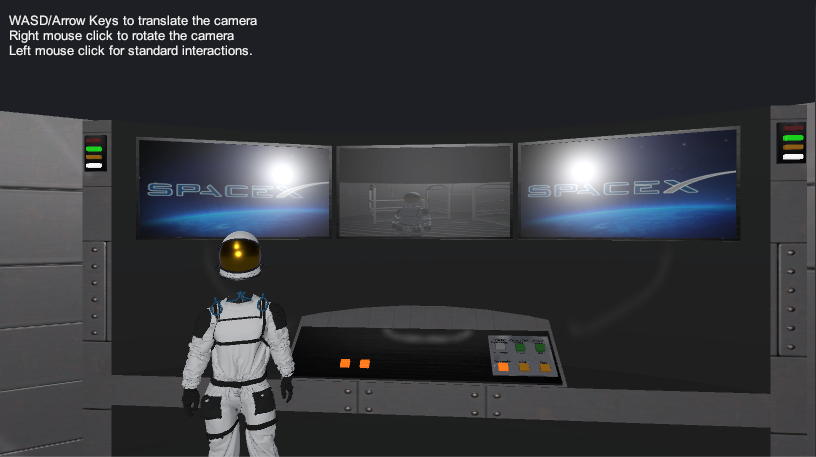
\includegraphics[width=0.8\textwidth]{VirgosScreenview.PNG}
\caption{Einer der Avatare, während seine Sicht auf dem Bildschirm dargestellt wird}
\end{figure}

\newpage

Eine Erweiterung der Funktion ist das Wechseln der primären Kamera auf die sekundäre Kamera des jeweiligen Benutzers. Dies ermöglicht es dem Kommandanten durch die Augen des Astronauten zu sehen und so genauere Anweisungen zu geben oder mögliche Probleme zu identifizieren die nicht über den Voice-Chat kommuniziert werden können. Durch einen Druck auf den zweiten Knopf kann die lokale primäre Kamera mit der sekundären Kamera getauscht werden, die aktuell auf dem Bildschirm angezeigt wird. Dies geschieht indem die primäre Kamera und gleichzeitig die Render-Textur der sekundären Kamera des jeweiligen Avatars deaktiviert werden. Somit wird das Bild der sekundären Kamera nicht mehr auf dem Bildschirm in der Anwendung angezeigt, sondern auf dem echten Bildschirm des Benutzers. 

\begin{figure}[H]
\centering
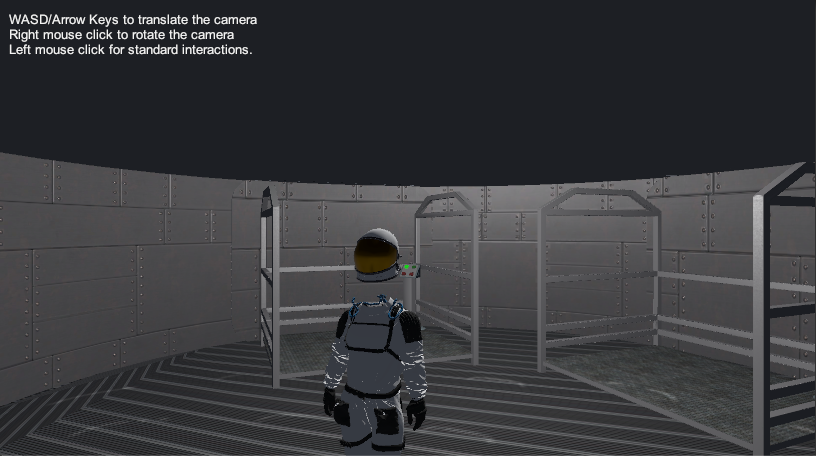
\includegraphics[width=0.8\textwidth]{ScreenDuplicate.PNG}
\caption{Die Sicht des Avatars, während sie den kompletten Bildschirm ausfüllt}
\end{figure}

\subsection{Einschränkungen durch Covid-19} \label{Covid}
Aufgrund der Covid-19-Pandemie und den daraus resultierenden Kontaktverboten und Schließungen von öffentlichen Einrichtungen, wirkte sich dies auch auf die Entwicklung dieses Projektes aus. Da sich das einzige verfügbare Virtual Reality Headset im Labor der Hochschule Reutlingen befand, erschwerte dies das Testen der Anwendung. Viele Funktionen konnten ohne Headset an einem Computer getestet werden, für Andere war das Testen mit einem Headset aber unumgänglich. Hierfür wurde mit einem Kommilitonen der Hochschule zusammengearbeitet, der privat über ein Headset verfügt. Dieser war freundlicherweise bereit die Anwendung in Virtual Reality zu testen und Besonderheiten oder Fehler über einen Voice-Chat zu schildern. Somit konnte zumindest regelmäßig auf Fehler reagiert, und diese behoben werden. \newline
Auch die Probandenbefragung war in der geplanten Form nicht durchführbar, da zum Zeitpunkt der Pandemie keine Vorlesungen in den Gebäuden der Hochschule gehalten wurden. Somit musste mit einer extrem verringerten Anzahl an Teilnehmern gearbeitet werden.
 
\section{Evaluation/Probandenbefragung} \label{Evaluation}
Fragebogen erklären, Ergebnisse darstellen, Erkenntnisse erläutern
\todo{Ergebnisse erklären}
\section{Fazit}
In diesem Kapitel wird im Rahmen der Diskussion zuerst auf die Anforderungen und die Testergebnisse eingegangen. Zum Abschluss werden im Unterkapitel Ausblick mögliche Erweiterungen und aktuelle Fehler in der Anwendung genannt, die in Zukunft implementiert und verbessert werden könnten.

\subsection{Diskussion} \label{Diskussion}
In dieser Diskussion werden zuerst die Anforderungen an die Arbeit aufgegriffen. Hierbei wird beschrieben ob die Anforderungen komplett, nur teilweise oder gar nicht umgesetzt werden konnten. Anschließend werden die Testergebnisse aus Kapitel \ref{Evaluation} zusammengefasst.

\subsubsection{Anforderungen}
Die meisten Anforderungen die in der Anforderungsanalyse definiert wurden konnten umgesetzt werden. Die Anforderung A1 \glqq Mehrere Benutzer gleichzeitig in der Anwendung\grqq{} wurde komplett umgesetzt. Die Anwendung kann von einem bis zehn Spielern gleichzeitig verwendet werden. Die Anwendung reagiert dynamisch auf das Beitreten und das Verlassen von Benutzern, ohne dass etwas angepasst oder neu gestartet werden muss.\\
Anforderung A2 \glqq Keine technische Abhängigkeit von einem VR-Headset\grqq{} wurde ebenfalls erfolgreich umgesetzt. Die Anwendung kann mit einem VR-Headset und dem Virtualizer oder über Maus und Tastatur benutzt werden. Welcher Spieler welche Technologie benutzt ist hierbei auch frei kombinierbar.\\
Die Rollen die in A3 \glqq Astronaut und Kommandant als Rollen für die Benutzer\grqq{} definiert wurden, wurden auch umgesetzt. Den Spielern werden keine festen Rollen zugewiesen, sondern von den Spielern dynamisch selbst gewählt. Dies geschieht durch die Positionierung in der Anwendung und die Benutzung der Werkzeuge, die für den Kommandanten gedacht sind.\\

A4 \glqq Informationsübertragung zwischen den Benutzern\grqq{} hingegen nicht komplett umgesetzt werden. Die sprachliche Kommunikation wurde bereits von der Basisanwendung angeboten. Die Position von anderen Spielern kann über den Bildschirm im Kontrollraum ermittelt werden. Mit der Funktion, die die Übernahme der Sicht eines anderen Spielers ermöglicht, können viele visuelle Informationen an den Kommandanten übermittelt werden. Die Funktionen für den Verweis auf Punkte im Raum und das Anbringen von Notizen konnten jedoch nicht umgesetzt werden. Abgesehen von dem Voicechat findet die Kommunikation aktuell folglich nur in eine Richtung von dem Astronauten zu dem Kommandanten statt.\\

\subsubsection{Testergebnisse}

Die Ergebnisse der Probandenbefragung die in Kapitel \ref{Evaluation} beschrieben wird, lassen aufgrund der geringen Anzahl der Probanden leider kaum Rückschlüsse zu. Hinzu kommen die zu simple Aufgabe an den Astronauten und die Funktionalitäten die zwar entworfen, aber nicht umgesetzt werden konnten. Somit lässt sich die gestellte Forschungsfrage FF1 aus Kapitel\ref{FF1} leider nur sehr eingeschränkt beantworten.\\

Die Antworten aus der Befragung legen nahe, dass ViRGOS inklusive seiner Erweiterungen eine solide Basis darstellt. Es bedarf aber scheinbar Verbesserungen in den Bereichen der Immersion und der Benutzbarkeit der Anwendung. Dies bezieht sich sowohl auf die Software, als auch die Hardware.\\

Bezüglich der Kooperation lässt sich sagen, dass beide Teilnehmer permanent visuelle Informationen über die Umwelt und die Aufgabe benötigen. Dies lässt sich daraus schließen, dass beide Kommandanten sofort die Kamera des Astronauten übernommen haben, sobald dieser den virtuellen Raum verließ und kein direkter Blickkontakt mehr möglich war. Eine Kooperation rein auf Basis von auditiver Kommunikation kann den Ablauf somit erschweren, da sich der Kommandant die virtuelle Umgebung des Astronauten vorstellen muss. Für eine möglich korrekte Vorstellung ist somit extrem viel auditive Kommunikation notwendig. Um die Forschungsfrage dieser Arbeit genauer beantworten zu können, ist ein weiterer Test mit mehr Probanden und einer überarbeiteten Version der Anwendung notwendig.

\subsection{Ausblick} \label{Ausblick}

Die Anwendung kann auf mehrere Arten erweitert und verbessert werden. Der Versuchsaufbau kann komplexer gestaltet werden, damit mehr Kooperation und Anleitung von Seiten des Kommandanten notwendig ist. Die Knöpfe die aktuell zur Anwendung kommen sind recht selbsterklärend, weshalb andere Eingabemöglichkeiten wie zum Beispiel Hebel, Schalter oder Tastenfelder verwendet werden könnten. Des Weiteren kann eine andere Art des Eingreifens für den Kommandanten implementiert werden. Aktuell kann der Kommandant über den Bildschirm die Sicht des Astronauten übernehmen, was ausreichend ist um den Astronauten durch die Aufgabe zu navigieren. Eine Erweiterung, die den Kommandanten zwingen würde diese Ansicht zu verlassen, wäre hilfreich um die Interaktivität für den Kommandanten zu steigern. Es gibt mehr Vorteile dass sich der Kommandant auch in der Anwendung befindet, wenn dieser den Astronauten durch aktives Eingreifen unterstützen muss.\\

Auch auf technischer Seite können Verbesserungen vorgenommen werden. Die Kollisionsvermeidung, die aktuell mit der Stoppuhr gelöst wird, führt zu manchen Problemen. Wenn mehrere Spieler gleichzeitig Knöpfe betätigen möchten wird dies von den zentralen Skripten als Kollision interpretiert und verhindert. Auch die Verwendung von Photons PUN 2 bietet Raum zur Verbesserung. Zwar bietet PUN alles was für die erfolgreiche Umsetzung der Anwendung notwendig ist, jedoch wird hierbei auf den Cloud-Service von Photon zurück gegriffen. Somit bestehen gewisse Abhängigkeiten und potentielle rechtliche Fragen, die umgangen werden könnten. Eine Alternative wäre Bolt, was ebenfalls von Photon entwickelt wurde. Statt auf einen Cloud-Service zuzugreifen würde hierbei einer der Clients als Host eingesetzt werden. Diesem Host würden die anderen Clients dann beitreten. Diese Variante würde unweigerlich neue Probleme aufwerfen, aber eine Unabhängigkeit von den Cloud-Servern von Photon bieten.\\

Wie in Kapitel \ref{Konzeption} erwähnt waren Werkzeuge für den Kommandanten geplant die leider nicht umgesetzt werden konnten. Somit kann die Anwendung um ein Werkzeug erweitert werden, mit dem die Benutzer auf Punkte im Raum verweisen können. Auch das Platzieren von Notizen kann hilfreich sein, wenn die Aufgabe hiervon Gebrauch machen kann. Auch über die in dieser Arbeit konzeptionierten Werkzeuge hinaus gibt es Möglichkeiten der Erweiterung. Die Knöpfe, die aktuell verwendet werden, fallen durch ihre leuchtenden Farben schnell auf, was die Interaktivität nahe legt. Falls weniger auffällige Objekte verwendet werden, wäre ein Werkzeug hilfreich, mit dem interaktive Objekte hervorgehoben werden. Ein Ansatz hierfür wurde in Kapitel \ref{Vorstudie} erwähnt. Zuletzt gibt es einen Bug in dem bestehenden Werkzeug mit dem die Kamera übernommen werden kann. Der in Kapitel ~\nameref{Evaluation} beschriebene Fehler verhindert eine Rotation der Kamera, wodurch die Orientierung in der Welt sehr viel schwerer fällt und die Nützlichkeit der Werkzeugs extrem eingeschränkt wird.

\newpage
\printbibliography[heading=bibintoc] 
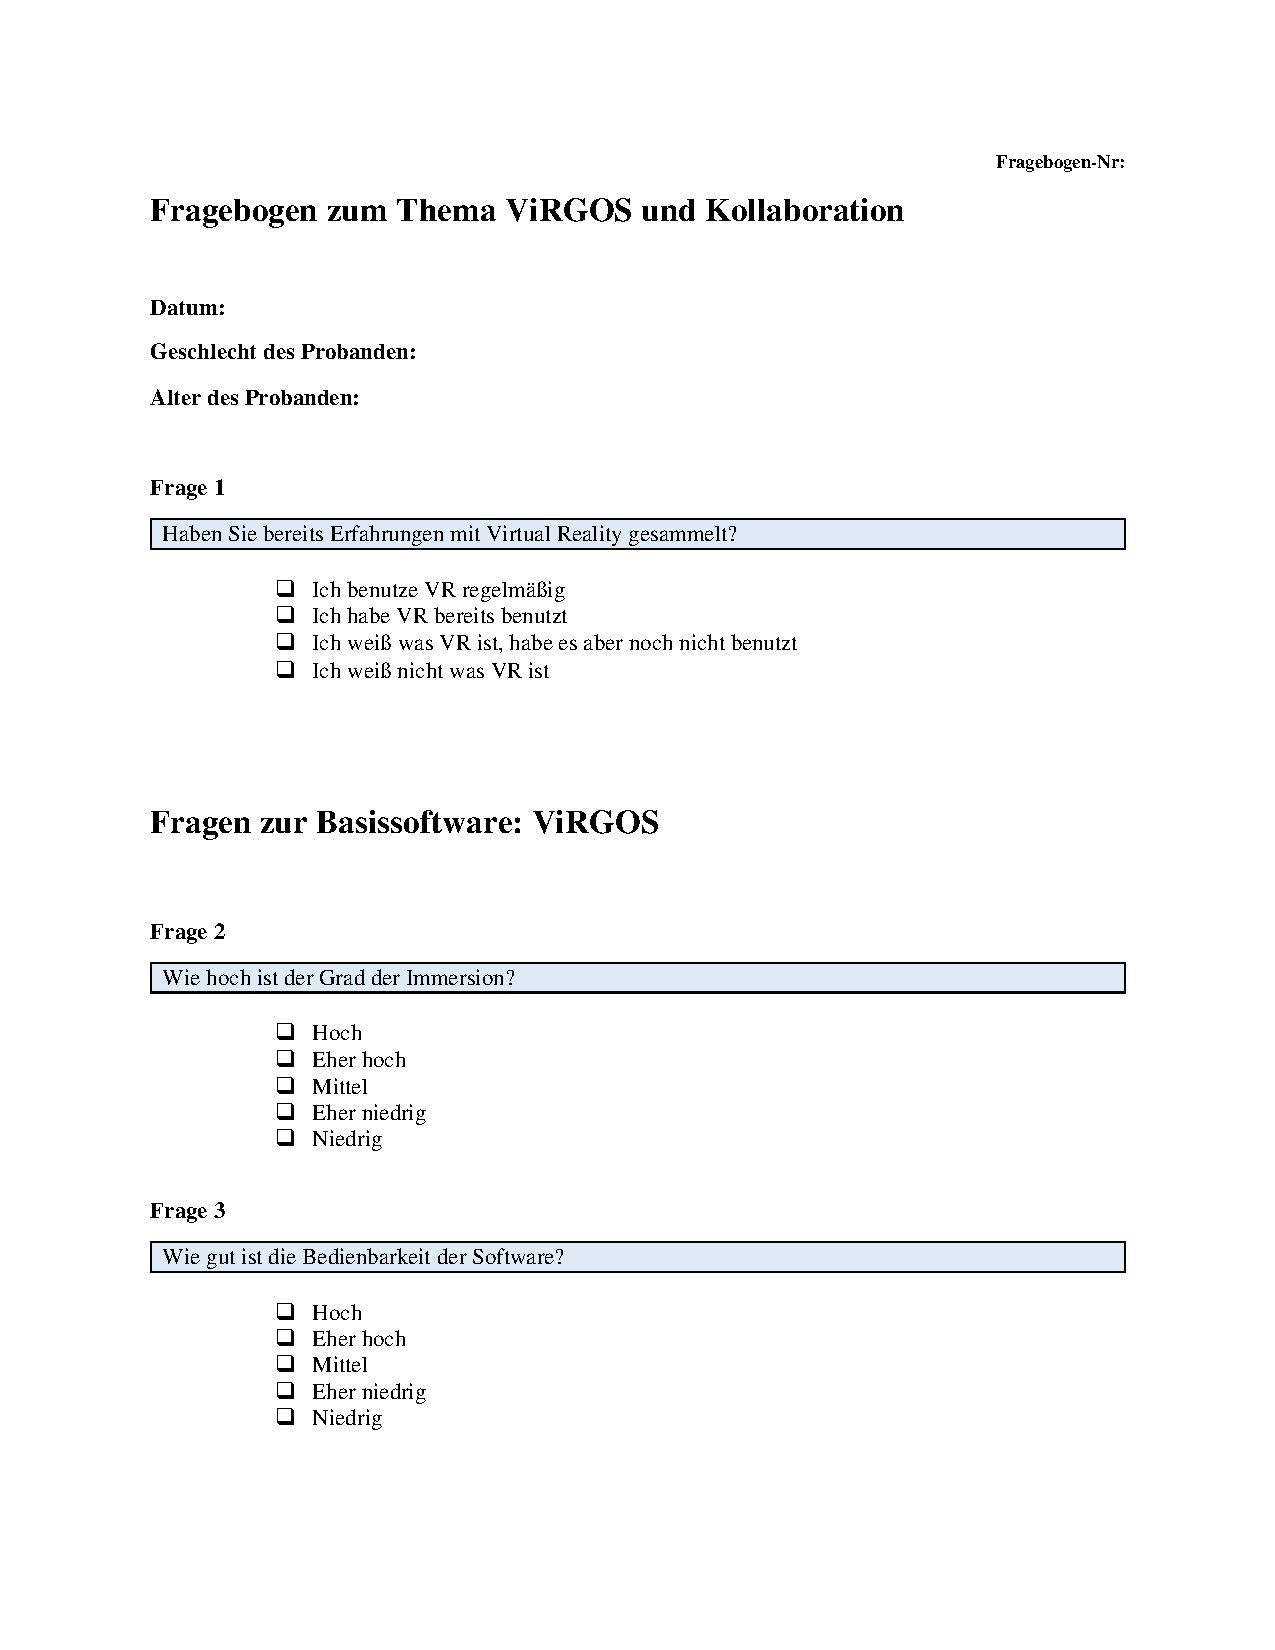
\includepdf[pages={1},scale=1, pagecommand=\section*{Anhang}]{ViRGOS_Fragebogen}\label{Anhang}
\includepdf[pages={2-},scale=1]{ViRGOS_Fragebogen}
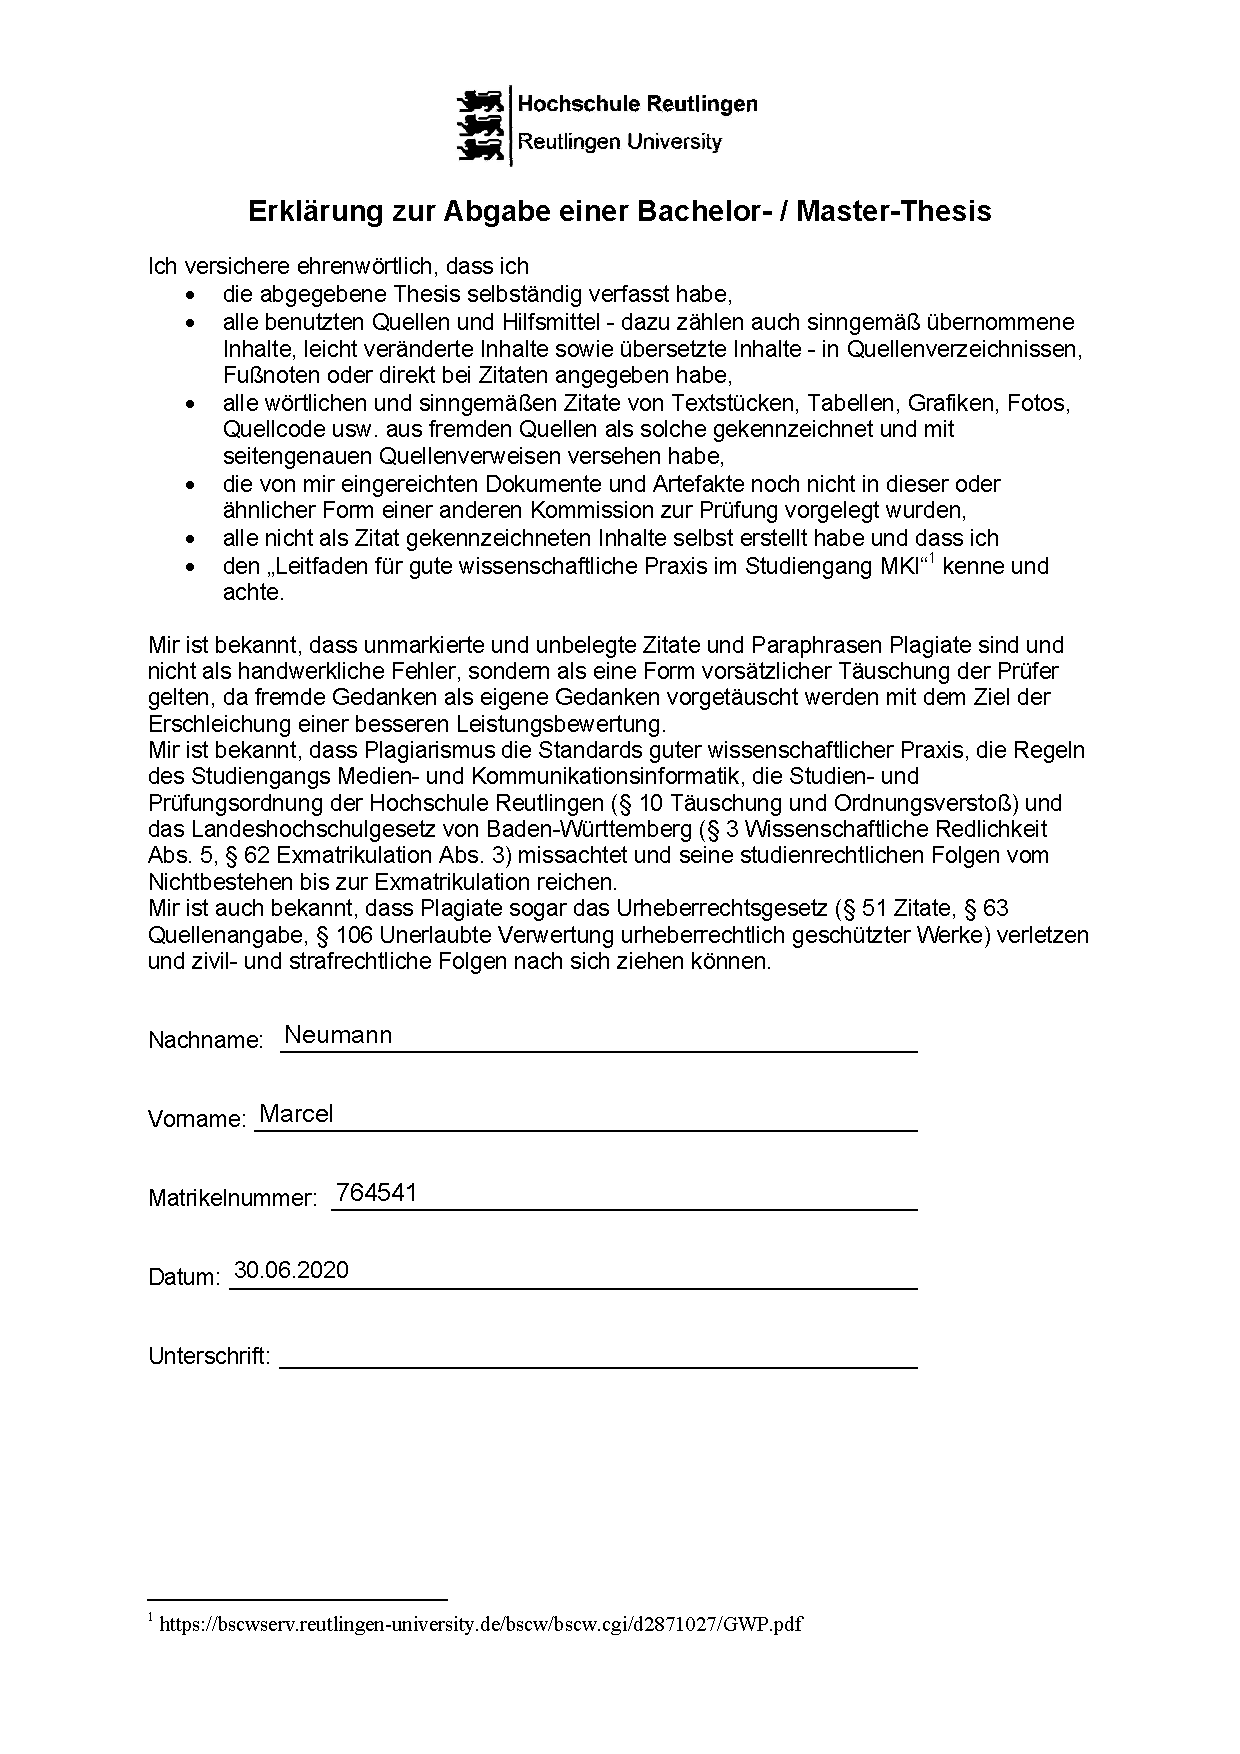
\includepdf{Erklaerung}
\end{document}